
%%%%%%%%%%%%%%%%%

\chapter{Data-Driven Sequential Learning  for Total Hedging Risk}
\label{sec:RNNTotal}
As we have discussed in section \ref{sec:DiscreteHedgingCriteria}, in reality, one often want to hedge until the expiry of the option. Total risk measures the hedging error from a dynamic hedging strategy in the entire hedging horizon. While mininimizing local risk has the effect of limiting the total hedging error, we investigate here whether minimizing the total hedging risk directly can lead to better total risk mimization strategy. From the model perspective, such enhancement is achievable. Indeed, recently a deep hedging model was proposed to minimize the total option hedging risk evaluated at the option expiry  \citep{buehler2019deep}. It is shown  that using a RNN to represent the hedging position model can be a computationally efficient framework to determine the optimal hedging function when the market is incomplete, e.g., under the transaction cost \citep{buehler2019deep}.

Although minimizing the total hedging risk, which is  the hedging portfolio value at the expiry $T$, is more desirable, there are several major obstacles in obtaining enough market data to build a data-driven total hedging model due to the fact that options listed in the exchanges often have fixed expiry dates (e.g., once a month for S\&P500 index options). The deep hedging model \citep{buehler2019deep} is only built on synthetic data. Due to the lack of market data needed to build a  model, applying the  deep hedging model \citep{buehler2019deep} can be challenging in real world applications.

In this chapter, we  provide a technique to deal with issue of lack of market data. In addition, an   sequential total risk hedging model $\modelT$ is introduced to minimize a discrete total risk hedging objective. We then build the total risk hedging model $\modelT$ based on the data augmentation technique we propose and demonstrate its effectiveness  and the performance of  the  total risk hedging model $\modelT$ using real market data experiments.  The goal in this chapter is to learn a hedging model for hedging option from a total hedging horizon of $N_H$ days to expiry. 


\section{Total Risk Hedging Model}
\label{sec:TotalModelDes}
In this section, we describe the total risk hedging model.
Figure \ref{fig:RNNModelTotal} depicts the proposed total risk GRU  hedging  model $\modelT$,
which is an extension from the local hedging model $\model$ we proposed in Chapter \ref{sec:RNNLocal}.
This model uses the sequential features, which encode information of two consecutive re-balancing time steps. In addition, the model uses the hedging position from the previous re-balancing time as the input. The output hedging position is used as the input for the next re-balancing time.



Following the discrete total risk definition in section \ref{sec:DiscreteTotalRisk}, consider a hedging portfolio  which is composed of:
\begin{itemize}
	\item A short position on option $V_{t,T,K}$.
	\item $\delta^{M}_{t,T,K}$ shares of $\Smkt_t$. 
	\item An amount in a risk-free bank account $B_t$.
\end{itemize}
% For the notational simplicity, we denote:
% \[
% \Vmkt_{t,T,K}=\Vmkt (t,T,K)\;,\Smkt_{t}=\Smkt(t)\;,B_t=B(t)\;, P^{H}_{t,T,K}=P^{H}_{t,T,K}
% \]
% Also, if $\Vmkt_{t,T,K}$ is not directly observable from market, it is set to be the  option prices from the parametrization of option value as discussed in section \ref{sec:DataAugmentation}. 
% Initially at $t_0$, we have
% \[
% P^H_{t_0,T,K}=  -V_{t_0,T,K}^{mkt}+\delta^{M}_{t_0,T,K} S_{t_0}+ B_{t_0}=0
% \]
% and
% \[
% B_{t_0}=V_{t_0}^{mkt}-\delta^{M}_{t_0,T,K} S_{t_0}
% \]
% Let us assume we rebalance $N_{rb}$ times until the expiry and the gap between each rebalancing time is fixed to be $\DT$:
% \[
% t_j=t_0+j \Delta t;\; j=0,\dots,N_{rb}-1;\;\;t_0=T-N_{rb}\DT
% \]
% At each rebalancing time $t_j$, we update our hedging position by changing the share we hold from $\delta^{M}_{t_{j}-\Delta t,T,K}$ to $\delta^{M}_{t_j,T,K}$ at $t_j$, where any required cash is borrowed, and any excess cash is loaned.
 As discussed in section \ref{sec:DiscreteTotalRisk}, the final hedging portfolio value at $T$ is:
 \begin{equation}
	\text{Risk}^{total}_{t_0,T,K}=\sum_{j=0}^{N_{rb}-1}\left\{ \left[\frac{\Smkt_{t_{j+1}}}{D(t_{j+1},T)}-\frac{\Smkt_{t_{j}}}{D(t_{j},T)}\right] \delta^M_{t_j,T,K} \right\}+\frac{V_{t_0,T,K}}{D(t_{0},T)}-V_{T,T,K}
	\label{eq:TotalRiskCh6}
\end{equation}
where
$D(t,T)=e^{-r(T-t)}$ is the discount factor and $\{t_0,t_1, \dots, t_{N_{rb}-1}\}$ is the set of rebalacing time. Note that, for testing scenarios, following the scenario construction procedure as in Algorithm \ref{alg:TestConstruction}, we can guarantee that $V_{t_0,T,K}$, $V_{T,T,K}$, and $\Smkt_t$ in equation \eqref{eq:TotalRiskCh6} are all directly from market instead of model.

Now, consider at a  rebalancing time $t \in \{t_0,t_1, \dots, t_{N_{rb}-1}\}$, with a strike $K$, and an expiry $T$. Assume we have computed the hedging position at the previous rebalancing time $t-\Delta t$: $\delta_{t-\Delta t, T,K}$. Let $\DT_{d}$ denote the time interval for sequential information recording. In  the subsequent empirical study, the interval $\DT_{d}$ equals one-day. Please note this setting is the same for local risk model described in Chapter \ref{sec:RNNLocal}.  We denote the sequential features recording the daily history  for hedging the option with expiry $T$ and strike $K$ as
\[
\mathbf{Y}_{t}^{T,K}=\left[\vy^{T,K}_{t-N \DT_{d}},\dots,\vy^{T,K}_{t}\right]
\]
For notational simplicity, we denote $\nt_i=t-(N+1-i)\DT_d$ with $i=1, \dots,N+1$, we thus have:
\[
\mathbf{Y}_{t}^{T,K}=\left[\vy^{T,K}_{\nt_{1}},\dots,\vy^{T,K}_{\nt_{N+1}}\right]
\]
The vector $\vy^{T,K}_{\nt_{i}} \in \Real^{d_s}$ has  $d_s$ features at time $\nt_{i}$ in the input sequential feature where
 $d_s$ is the dimension of the sequential feature $\mathbf{Y}_{t}^{T,K}$, and
$N+1$ is the length of the sequential feature sequence. We set $N=\frac{\Delta t}{\Delta t_d}$. Thus $\mathbf{Y}_{t}^{T,K}$ contains the sequential information in between two consecutive rebalancing time $t$ and $t-\Delta t$.
The encoder transforms information from the sequential feature $\mathbf{Y}_{t}^{T,K}$ to  a fixed-sized vector
$\mathbf{\widehat{h}}_E$   and the decoder makes the final prediction based on both $\mathbf{\widehat{h}}_E$  and the previous hedging position $\delta^{M}_{t-\Delta t,T,K}$. The overall structure of the proposed model is illustrated in Figure \ref{fig:RNNModelTotal}. Note that for the initial hedging date $t=t_0$, the previous hedging position is set as $0$.



\begin{figure}[htp!]
	\centering
	\resizebox{0.65\textwidth}{!}{
		\begin{tikzpicture}[
		prod/.style={circle, draw, inner sep=0pt},
		ct/.style={circle, draw, inner sep=5pt, ultra thick, minimum width=10mm},
		ft/.style={circle, draw, minimum width=8mm, inner sep=1pt},
		filter/.style={circle, draw, minimum width=7mm, inner sep=1pt, path picture={\draw[thick, rounded corners] (path picture bounding box.center)--++(65:2mm)--++(0:1mm);
				\draw[thick, rounded corners] (path picture bounding box.center)--++(245:2mm)--++(180:1mm);}},
		mylabel/.style={font=\scriptsize\sffamily},
		>=LaTeX
		]
		
		
		\node[draw,rectangle]  (s1) at (4.5, -3) {softmax};
		\node[draw,rectangle]  (s3) at (7.5, -3) {softmax};
		\node [inner sep=0pt] (rp1) at (3*1, -3) {$\odot$};
		\node  (rp2) at (3*2, -1.5) {$\dots$};
		\node [inner sep=0pt] (rp3) at (3*3, -3) {$\odot$};
		
		\foreach \i [count=\step from 1] in {$\vy^{T,K}_{\nt_{1}}$,$\dots$,$\vy^{T,K}_{\nt_{N+1}}$}
		\node (ri\step) at (3*\step, -4) {\i};
		\node  (sw1) at (4.5, -4) {$\omega^S$ };
		\node  (sw3) at (7.5, -4) {$\omega^S$};
		\draw[->] (s1.west) to node[below]{} (rp1.east);
		\draw[->] (s3.east) to node[below]{} (rp3.west);
		\draw[->] (ri1.north) to (rp1.south);
		\draw[->] (ri3.north) to (rp3.south);
		\draw[->] (sw1.north) to (s1.south);
		\draw[->] (sw3.north) to (s3.south);
		\node (h2) at (3*2, 0.0) {$\dots$};
		\foreach \step in {1,3} {
			\node[draw,rectangle] (h\step) at (3*\step, 0.0) {GRU};
		}
		\draw[->] (rp1.north) to node[right]{$\widehat{\vy}^{T,K}_{\nt_{1}}$} (h1.south);
		\draw[->] (rp3.north) to node[left]{$\widehat{\vy}^{T,K}_{\nt_{N+1}}$} (h3.south);
		
		%\draw[->] (i4) -> (h4.south);
		\draw[->] (h1.east) to node[below]{$\vh_1$} (h2.west);
		\draw[->] (h2.east) to node[below]{$\vh_{N}$} (h3.west);
		%\foreach \step in {1,...,2} {
		%	\pgfmathtruncatemacro{\next}{add(\step,1)}
		%	\draw[->] (h\step.east) -> (h\next.west);
		%}
		\node[fit=(ri1) (ri3) (s1) (s3) (h1) (h3), draw, inner sep=0pt] (fit1) { };
		\node[align=center, outer sep=0] (encoder) [right=of fit1] {Encoder};
		
		
		
		\node[filter] (oe2) at (9, 4.5) {};
		\node[filter] (oe3) at (6, 4.5) {};
		\node [inner sep=0pt] (oe4) at (6, 6.5) {$\odot$};
		\node [inner sep=0pt] (oe5) at (9, 6.5) {$\odot$};
		\node [draw,circle,inner sep=0pt] (oe6) at (7.5, 7.5) {$+$};
		\node (oe7) at (7.5, 8.5) {$\delta^M_{t,T,K}$};
		\node  (bs) at (4.5, 6.5) {$\delta^{BS}_{t,T,K}$};
		\draw[->] (oe3.north) to node[left]{$1-W_{\delta} $} (oe4.south);
		\draw[->] (oe3.north) to node[above]{$W_{\delta}$} (oe5.west);
		\draw[->] (oe2.north) to node[left]{$\widehat{\delta}^M_{t,T,K}$} (oe5.south);
		\draw[->] (oe4.north) to node[left]{} (oe6.west);
		\draw[->] (oe5.north) to node[left]{} (oe6.east);
		\draw[->] (oe6.north) to node[left]{} (oe7.south);
		\draw[->] (bs.east) to node[left]{} (oe4.west);
		
		
		

		
		\node[inner sep=0pt]  (l1) at (6, 1) {$\delta^M_{t-\Delta t,T,K}$};
		\draw[->] (1, 1) to node[above]{output from $t-\Delta t$} (l1.west);

		
		\node (he2) at (6, 3) {$\delta^M_{t-\Delta t,T,K}$};
		\node (he3) at (9, 3) {$\widehat{\mathbf{h}}_E$};
		\draw[->] (l1.north) to (he2.south);
		\draw[->] (h3.north) to  (he3.south);
		\draw[->] (he3.north) to  (oe2.south);
		\draw[->] (he3.north) to  (oe3.south);
		
		\draw[->] (he2.north) to (oe2.south);
		\draw[->] (he2.north) to (oe3.south);
		
		\node[fit=(oe2) (oe3) (oe5) (oe6)  (oe7)  (bs) (he2) (he3), draw, inner sep=0pt] (fit3) { };
		\node[align=center, outer sep=0] (encoder) [left=of fit3] {Decoder};

		\draw (oe7.north)  to (7.5,10) to (10.5,10) to node[right]{$\delta^M_{t,T,K}$} (10.5,1);
		\draw[->] (10.5,1) to node[above]{input to $t+\Delta t$} (13.5,1);

		\end{tikzpicture}
	}
	\caption{$\modelT$: GRU encode-decoder total hedging model. The encoder summarizes the time series $\mathbf{Y}_{t}^{T,K}=\left[\vy^{T,K}_{\nt_{1}},\dots,\vy^{T,K}_{\nt_{N+1}}\right]$ as a succinct  vector $\widehat{\mathbf{h}}_E$. The decoder outputs the hedging position based on the vector $\widehat{\mathbf{h}}_E$ and the previous hedging position $\delta^M_{t-\Delta t,T,K}$ observed at the hedging time $t$. More specifically, in the decoder, a candidate output $\widehat{\delta}^M_{t,T,K}$ is firstly produced. The final output $\delta^M_{t,T,K}$ is computed based on the linear combination of BS delta $\delta^{BS}_{t,T,K}$ and the candidate output  $\widehat{\delta}^M_{t,T,K}$. The combination weight is determined by  $W_{\delta}$. The feature weight $\omega^L$ is used to compute weighted sequential feature $\widehat{\vy}^{T,K}_{\nt}$. The weighting acts as a feature selection process.
		Each edge in the graph has an arrow on it, pointing from a node whose output is used by the node pointed by the arrow as an input. The output $\delta^M_{t,T,K}$ at $t$ is used as the input for next step $t+\DT$.}
	\label{fig:RNNModelTotal}
\end{figure}



\subsection{Difference Between  $\model$ And $\modelT$}
Comparing  $\model$  in Figure \ref{fig:RNNModel} and  $\modelT$  in Figure \ref{fig:RNNModelTotal}, it is clear that the model structures between $\model$ and $\modelT$ are similar. 
 The most significant difference between  $\modelT$ and  $\model$ is that $\model$ is built on minimizing discrete local risk as in section \ref{sec:DiscreteLocalRisk} while $\modelT$ is built based on minimizing the discrete total risk as in in section \ref{sec:DiscreteTotalRisk}.

More differences between $\modelT$ and $\model$ are given below:
\begin{itemize}
	
\item In $\model$, we have a local features vector $\vx^{T,K}_{t} \in \Real^{d_l}$ which records local information at the hedging time $t$ for hedging the option with expiry $T$ and strike $K$. In Chapter \ref{sec:RNNLocal} we demonstrate importance of using sequential learning by  comparing performance with and without sequential features. 

\item Recognize importance of sequential features, in $\modelT$, here we omit the local features vector $\vx^{T,K}_{t} \in \Real^{d_l}$ as the input to the model $\modelT$ and use the sequential feature  $\mathbf{Y}_{t}^{T,K}$ which contains all the sequential information between two consecutive rebalancing time $t$ and $t-\DT$. 
Note that sequential feature also contains the local information the the hedging time $t$.

\item Since the analytical formula for the variance-optimal total risk hedging \cite{schweizer1995variance} and spline total risk minimization formulation \cite{coleman2007total} both  demonstrate the dependence of the current hedging position on the past hedging position, we include previous hedging position $\delta^{M}_{t-\Delta t,T,K}$ as the input to compute the current hedging position $\delta^{M}_{t,T,K}$. 
	
%	Additionally, we have conducted a set numerical comparisons under synthetic scenarios between $\modelT$,  the  spline total risk minimization formulation \cite{coleman2007total} and  variance-optimal total risk hedging formulation \cite{schweizer1995variance}. We demonstrate that $\modelT$ can produce equivalent hedging performance under Black-Scholes synthetic scenarios when comparing with the models in  \cite{coleman2007total} and \cite{schweizer1995variance}. More details on the comparison can be found in Appendix \ref{sec:SynCompara}.
\end{itemize}

The more details of the  model structure of $\modelT$ is discussed in Appendix \ref{App:modelstructure}.


\subsection{Training Objective For $\modelT$}
\label{sec:TotalModelObj}
Assume that we are given  a set  of hedging scenarios identified by the expiry date $T_i$ and strike $K_i$:
\[
\{Scenario(T_1,K_1), \dots, Scenario(T_M,K_M)\}	
\]
% Additionally, we denote  the set of rebalacing date identified by starting date $t_0$, expiry date $T$ and rebalacing frequency $\Delta t$ by $\mathbf{t}_{rb}(t_0, T,\Delta t)$:


A natural total risk hedging loss function is the mean squared error:
\[
MSE_{total}=\frac{1}{M} \sum_{i=1}^M  (\text{Risk}^{total}_{t_0^i,T_i,K_i})^2
\]
where $\text{Risk}^{total}_{t_0,T,K}$ is defined as in equation \eqref{eq:TotalRiskCh6},  $t_0^i=T_i-\frac{100}{250}$, and $M$ is the number of hedging scenarios.
A more appropriate criteria however is the relative hedging error instead of the absolute total hedging error since we are mixing scenarios of different strikes together (i.e., the scenarios include near-money, in-the-money, and out-of-the money options. The absolute hedging error for in-the-money options tend to be much bigger than those of  near-the-money options and out-of-money options). Additionally, MSE is sensitive to the existence of outliers. Furthermore, \citet{coleman2007total} demonstrated that the  $l_1$-norm error loss function can produce better hedging performance. 
Therefore, in training the $\modelT$, we use the following objective:
\begin{equation}
Obj_{total}=\sum_{i=1}^M \left|\text{Rel}^{total}_{t_0^{i},T_i,K_i}\right|
\label{eq:totalObjLinear}
\end{equation}
where the relative total hedging error is defined as:
\begin{equation}
	\text{Rel}^{total}_{t_0,T,K}
	=\frac{D(t_0,T_i)  \text{Risk}^{total}_{t_0,T,K}}{V_{t_0,T,K}}
	\label{eq:relHError}
\end{equation}


%Since $\model$ is built on top of pure market data while $\modelT$ is built on top of augmented market data, we will not compare the performance of  $\model$ and $\modelT$ directly. Since, here we are more interested in the effect of the choice of objective functions. Therefore, we define a new comparing model $\modelL$. The model structure of $\modelL$ is exactly the same as  $\modelT$ which is as in Figure \ref{fig:RNNModelTotal}.  The only difference is $\modelT$ is built on minimizing objective \eqref{eq:totalObjLinear}. While the $\modelL$ is built on minimizing a local risk objective.
%
%More specifically, for an expiry $T$ and a strike $K$,  at a rebalancing time $t_j$ ,we have
%
%\[
%\begin{split}
%\Delta V^{mkt}_{t_j,K,T}& =D(t_0,t_{j+1}) V^{mkt}_{t_{j+1},K,T}-D(t_0,t_{j})V^{mkt}_{t_j,K,T}\\
%\Delta \Smkt_{t_j} &=D(t_0,t_{j+1}) \Smkt_{t_{j+1}}-D(t_0,t_{j}) \Smkt_{t_{j}}\\
%&D(t,T)=e^{-r(T-t)}\\
%\end{split}
%\]
%\[
%t_j=t_0+j \Delta t;\; j=0,\dots,N_{rb}-1;\;\;t_0=T-N_{rb}\DT
%\] 
%If the option price $V^{mkt}_{t,K,T}$ is not directly observable from market, we will use the model prices from the parametrization we calibrated as the replacement.
%The objective for the  $\modelL$  is therefore:
%\begin{equation}
%Obj_{Local}=\sum_{i=1}^M \sum_{t\in t_{rb}(t_0^i, T_i,\Delta t)} |\Delta V^{mkt}_{t,T^i,K^i}-\DS_{t} \delta^{M}_{t,T^i,K^i}|
%\label{eq:LocalObjNew}
%\end{equation}

\subsection{Market Data Augmentation}
\label{sec:DataAugmentation}
As discussed in section \ref{sec:DiscreteTotalRisk}, the final hedging portfolio value at $T$ is:
\begin{equation}
   \text{Risk}^{total}_{t_0,T,K}=\sum_{j=0}^{N_{rb}-1}\left\{ \left[\frac{\Smkt_{t_{j+1}}}{D(t_{j+1},T)}-\frac{\Smkt_{t_{j}}}{D(t_{j},T)}\right] \delta^M_{t_j,T,K} \right\}+\frac{V_{t_0,T,K}}{D(t_{0},T)}-V_{T,T,K}
\end{equation}
where
$D(t,T)=e^{-r(T-t)}$ is the discount factor and $\{t_0,t_1, \dots, t_{N_{rb}-1}\}$ is the set of rebalacing time. The $t_0$ in this thesis is set to be $N_H$ days to the expiry where $N_H$  is a constant. 

\iffalse  %suggest delete, repeat
Suppose we have $M$ hedging scenarios, a data driven model can be built by minimizing total hedging loss function such as MSE:
\[
    MSE_{total}=\frac{1}{M}\sum_{i=1}^M  (\text{Risk}^{total}_{t^i_0,T_i,K_i})^2
\]
Clearly, in order to build an effective data-driven total risk hedging model, one needs to gather a sufficient  number $M$ of sample paths. 

For local risk hedging, each data instance is uniquely determined by the triplet $\{t,T,K\}$. We only need the market option prices of strike $K$ and expiry $T$ to be available on both $t$ and $t+\Delta t$ to gather a data instance for the data-driven local hedging model. Therefore, purely building a model based on market prices for local risk hedging is achievable. When we build the local risk hedging model, the time to maturity $\tau=T-t$ is not fixed.
\fi

For total risk hedging, if we assume the starting hedging date $t_0$ is $N_H$ days to expiry $T$, each data instance is then uniquely determined by the duplet $\{T,K\}$. If we only rely on market prices to build the total risk model,  we will face the following challenges:
\begin{enumerate}
		\item Options listed in an exchange only have fixed expiry dates and only a few strikes are listed every day. In other words, the number of unique duplet $\{T,K\}$ in actual market is small.		
		For example, the expiration date for the standard S\&P 500 index option is fixed at the third Friday of each month.\footnote{Starting from 2016, CBOE also introduces weekly S\&P 500 index options which expired on Monday, Wednesday and Friday of each week. The data we gathered is up to 2015-08-31, so our experiments in this thesis does not include those data.} Therefore, if we only use market available expiration dates, the number of training scenarios will  be severely limited. 
		\item In addition, the option with specific strike $K$ and expiry $T$ may not be traded  on every trading date during its lifetime. Requiring the market option prices of strike $K$ and expiry $T$ to be available on entire hedging horizon $[t_0, T]$ is unrealistic especially for in-the-money and out-of-money options. 
		Therefore, we will have to rely on certain parametric models calibrated to market prices to compute the necessary derived features (e.g., option sensitivity), which is used as the input of the data-driven model, when there are not market prices for the specific combination of $T$ and $K$ on some trading dates.
		\item Lastly, under an ideal setting, one should  use non-overlapping underlying asset paths to generate training and testing hedging scenarios as one often observe autocorrelation in financial time series.  In reality, using non-overlapping underlying asset path to generate training and testing scenarios is not practical. For instance, assuming we are building a data-driven model for hedging 3
		months until expiry, with non-overlapping underlying asset paths, 20 years of market data can provide only 80 different non-overlapping underlying asset paths, making building a
		data-driven model difficult.  
\end{enumerate}


In order to overcome  above challenges, we propose the following remedy.  
\begin{enumerate}
	\item Overlapping underlying asset paths are allowed.
	\item A no-arbitrage  surface is calibrated on each business day to match the market prices. We will query the calibrated surface to obtain the option prices and option sensitivities when the corresponding market data is not available. 
	\item Instead of using only market available expiration dates, we assume every business day can be the expiration date of the options. The option prices and option sensitivities for these newly added expiry dates will come from querying the no-arbitrage  surface.
\end{enumerate}


Therefore, we greatly increase the number of training scenarios, since now the hedging scenarios can have more combinations of $T$ and $K$ even if the combinations of $T$ and $K$ are not directly observed in the market. 
We create a parametrization of the price surface that is \textbf{arbitrage-free}.  This is done by using SABR model to match the market volatility smiles and we use an arbitrage-free interpolation based on Local Volatility Function (LVF) model to interpolate the SABR model value between expiries.


As an example, in Figure \ref{fig:CaliExp}, we show the resulting price surface and implied  volatility surface for SP500 index call options  on 2012-01-04. In Figure $\ref{fig:CaliExp}$, we use $\tau=T-t$ to denote the time to maturity.  


\begin{figure}[htp!]
	\centering
	\subfigure[Implied  Volatility Surface]{
		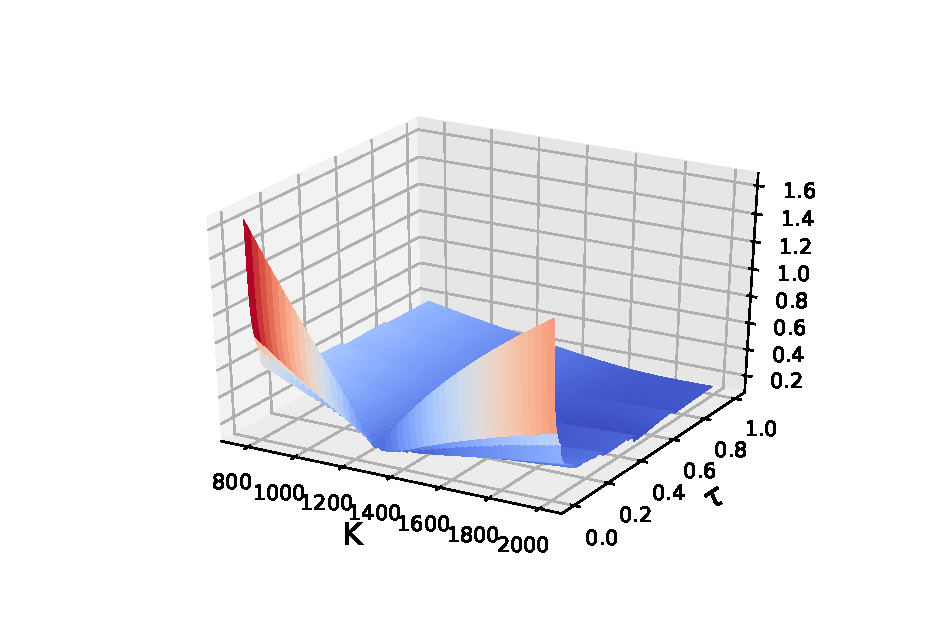
\includegraphics[width=0.8\textwidth]{./figures/ImpVol}
	}
	\subfigure[Price Surface]{
		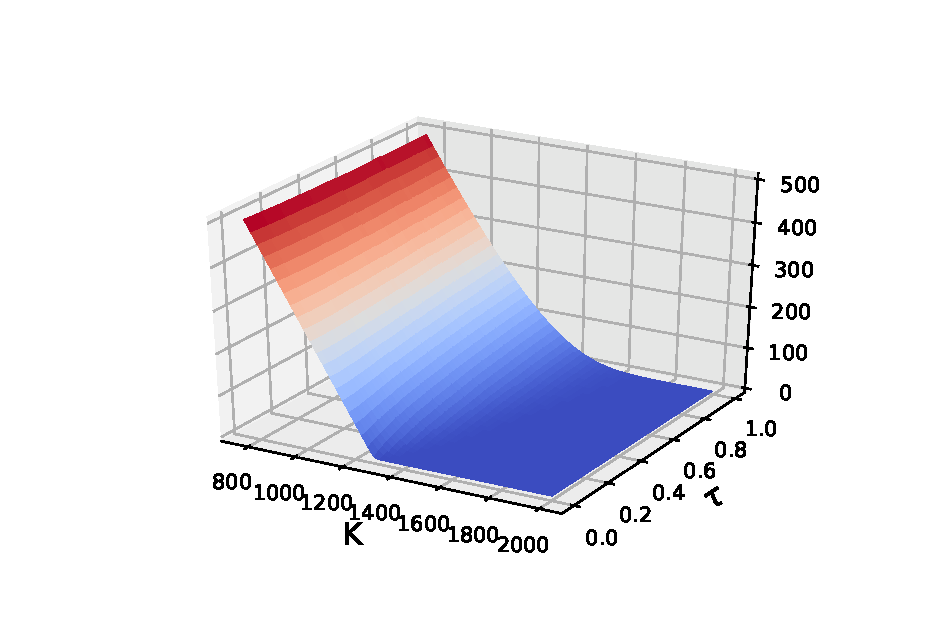
\includegraphics[width=0.8\textwidth]{./figures/Price}
	}
	\caption{The price surface and implied volatility surface calibrated to SP500 index call options on 2012-01-04. The smile is more pronounced for the shorter maturities than the longer maturities, which is consistent with observations from various studies \cite{chance2017bias,rogers2010can} using market data. Interested readers can also refer to \cite{rogers2010can} for some mathematicaly explaination on why the smile becomes more and more flattened as $\tau$ increases.}
	\label{fig:CaliExp}
\end{figure}

We refer an interested reader to Appendix \S \ref{sec:NoArb} for details of no arbitrage surface calibration.

\subsection{Training and Testing Data Construction}
\label{sec:Augtrain}

In this section, we will discuss the training and testing data construction for building the total hedging model with the surfaces constructed from SABR and LVF model. The training and testing data set are the collection of hedging scenarios. Each of the hedging scenarios is identified uniquely by a duplet of expiry date and strike  $(T,K)$. \footnote{ If we fixed the gap between two rebalancing time to be $\DT$ and we fix the number of times we rebalance the hedging portfolio to be $N_{rb}$, then given an expiry $T$, one can easily deduct the rebalance time $\{t_0,t_1, \dots, t_{N_{rb}-1}\}$ . Therefore, we can uniquely define a hedging scenario just by $T$ and $K$.} Let $t_0$ be the initial date to set up the hedging portfolio and $\mathbf{t}_B=\{t_0,\dots,T\}$ be the set of all business days in between the initial date $t_0$ and expiry date $T$.  Each of the hedging scenarios is the collection of the following time series identified uniquely by $(T,K)$:
\begin{itemize}
	\item $\{S_t|\forall t \in \mathbf{t}_B \}$: the the time-series of underlying prices  with $t_0$ as the initial date and $T$ as the expiry date.
	\item $\{V_{t,T,K}|\forall t \in \mathbf{t}_B\}$:  the time-series of option value for a hedging scenario identified by $(T,K)$.
	\item $\{\vy^{T,K}_{t}|\forall t \in \mathbf{t}_B\}$: the time-series of feature vectors for a hedging scenario identified by $(T,K)$.
\end{itemize}


\subsubsection{Construction of Training Scenarios}
Based on the calibration process we discussed above, we summarize the procedure for generating training scenarios for hedging $N_H$ business days as the following. \begin{enumerate}
	\item Each of the hedging scenarios is identified uniquely by a duplet of expiry and strike  $(T,K)$. We need to construct the time series corresponding to the duplet as the input to our model. For a training scenario, we do not require the option prices for the  duplet $(T,K)$ to exist in market. We will query the surface constructed by Algorithm \ref{alg:SurfaceConstruction} for each time $t$: $V_{model}^t(T,K)$ for option values and compute the associated option related sensitivities, which are used to construct the feature vector for the model. In this way, we greatly increase the number of training scenarios.  
	\item The starting date $t_0$ to set up the initial hedging portfolio is  $N_H$-business days away from the expiry date $T$. In this thesis,  $N_H$ is set to be 100.  We assume there are 250 business days in a year. Denote $T_{t,max}^{mkt}$ as the maximum expiry listed in exchange at time $t$. We further comment that we always have $T_{t,max}^{mkt}-t>100/250$ in market for all the business dates we include in the experiments.  Therefore, no volatility extrapolation is needed.
	\item We check all the market observed strikes for all the business dates between $t_0$ and  $T$. Let $K^{mkt}_{max}(t_0,T)$ be the maximum of  strikes we observed in market  between $t_0$ and  $T$. The grid of strikes for the outputting option values with expiry date $T$ is defined as: $\mathbf{K}_{grid}(t_0,{T})=\{0=K_0<K_1<\dots<2*K^{mkt}_{max}(t_0,\widehat{T})\}$ where $K_i-K_{i-1}=\Delta K, i \geq 1$. In this chapter, we set $\Delta K=5$ for experiments on S\&P 500 index options which is consistent with the S\&P500 index option strike specification in real market \cite{hull2006options}.
%	\item On each business day $t \in [t_0,\widehat{T})$, following the calibration process in section \ref{sec:NoArb}, we  obtain a parametrization of the option value:$\{V_{t}(T,K)\}_{T,K}$. We then query $\{V_{t}(T,K)\}_{T,K}$ to obtain  option related information such as option prices and option sensitivities. For example, for each $K \in \mathbf{K}_{grid}(t,\widehat{T})$, we extract option value by $V_{t}(\widehat{T},K)$ at each business $t \in [t_0,\widehat{T})$, therefore, we obtain the time series of option values from $t_0$ to $\widehat{T}$ for each $K$.
%	\item The time series of underlying prices $S_t$  are obtained directly from market. 
\end{enumerate}
A detailed description is given in Algorithm \ref{alg:Construction} in Appendix \S \ref{}.

\subsubsection{Construction of the Testing Scenarios}
\label{sec:AugTest}
The key differences between the testing scenarios and the training scenarios are:
\begin{itemize}
	\item  For testing scenarios, we use real market prices to initialize the hedging portfolio at $t_0$ and the strikes and expiries are real market strikes and expiries.
	\item  For testing scenarios, we use real option market data to construct the time-series whenever associated  option market data is available. Otherwise, we will query the calibrated option value function.
	\item For training scenarios, we use model prices to initialize the hedging portfolio. The strikes and expiries do not necessarily have to be are real market strikes and expiries.
	\item   For training scenarios, we always query the parametrization of the option value we calibrated to construct  the time series. Please note that  since we calibrate the models to match the market prices, when market prices are available, the model prices will be very close to the market prices. 
\end{itemize}
A summary of the construction of testing scenarios is as the following. A detailed algorithm is given in Algorithm \ref{alg:TestConstruction}.

\begin{enumerate}
	\item A testing expiry date $T$ must be a real expiry date that exists in market. Before 2016, For the S\&P 500 index options listed in Chicago Board Options Exchange (CBOE) the expiration dates are the third Fridays of each month. After 2016, more expiration dates are introduced in CBOE.
	\item The date $t_0$ to set up the initial hedging portfolio is  $N_H$-business days away from $T$.
	\item On the starting date $t_0$, we can obtain all market option prices for the expiry  $T$ and we have a grid of market strikes for expiry $T$ on date $t_0$:
	$\mathbf{K}^{mkt}_{grid}(t _0,T)=\{	K^{mkt}_{t_0,T,1},\dots,K^{mkt}_{t_0,T,N_K}\}$. Note that we have market options  prices for all $K \in \mathbf{K}^{mkt}_{grid}(t _0,T)$ at time $t_0$.
	\item On each business day $t$ in between $t _0$ and $T$, an arbitrage free surface is constructed $\{V^{t}_{model}(T,K)\}_{T,K}$ using Algorithm \ref{alg:SurfaceConstruction}. 
	When there is no  market price $V^{mkt}_{t,T,K}$ on time $t$ for $K \in \mathbf{K}^{mkt}_{grid}(t _0,T)$, we will query $\{V^{t}_{model}(T,K)\}_{T,K}$ to obtain  option prices and option sensitivities.  Note that, with this approach, for instance, a part  of the time series of option prices for a testing scenario can be real market prices while the other part can be model prices from the  parametrization  obtained following the calibration process in section \ref{sec:NoArb}.
	% The grid for testing is set to be $\mathbf{K}^{test}_{grid}=\{K_0=0<K_1<\dots<K_{max}\}$ where $K_i-K_{i-1}=\Delta K, i \geq 1$ and $K_{max}=2 \times K^{mkt}_{N_K}$. Please note that $\mathbf{K}^{mkt}_{t_0,T_{test}} \subset \mathbf{K}^{test}_{grid}$.  
	% \item On each business day $t \in [t,T_{test})$, we can observed a set of market observed expiries: $\mathbf{T}_t^{mkt}=\{T_0^{t},T_1^{t},\dots,T_{max}^{t}\}$.
	% 	\item  We calibrate the SABR models for each market observed expires $T_i^{t} \in \mathbf{T}_t^{mkt},	\;  t \in [t_0, T),T \in \mathbf{T}_t^{mkt}$. The calibrated SABR models return the prices  for the grid of strikes and we fix the potential arbitrages for SABR prices returned by the SABR models, if there is any. 
	% 	\item If $T_{test} \in \mathbf{T}_t^{mkt}, K \in \mathbf{K}^{mkt}_{t_0,T_{test}}$,  and $\Vmkt_{t,T_{test},K}$ is directly observable from market. 
	% We will just use the market data to construct the time series needed for the hedging model. 
	% 	\item If $T_{test} \in \mathbf{T}_t^{mkt}, K \in \mathbf{K}^{mkt}_{t_0,T_{test}}$ but  the 
	% $\Vmkt_{t,T_{test},K}$ is not directly observable from market, we will use SABR model to fill the gaps. In this case,we assume  $\Vmkt_{t,T_{test},K}=V^{SABR}_{t,T_{test},K}$.
	% \item
	% If  we do not have enough data to calibrate a SABR model for $T_{test} \in  \mathbf{T}_t^{mkt}$, we can use the  volatility interpolation process \cite{andreasen2010volatility} to obtain option prices on each day $t$ for the expiry $T_{train}$ we picked on step 1: $V^{LVF}_{t,T_{test},K}$ where $t \in [t_0, T_{test}), K \in \mathbf{K}^{mkt}_{t_0,T_{test}}$.  In this case, we assume $\Vmkt_{t,T_{test},K}=V^{LVF}_{t,T_{test},K}$. Furthermore, we can also obtain other option related information such as Black-Scholes delta, gamma, vega and so on.
\end{enumerate}

\subsubsection{Construction of Training, Testing and Validation Data Sets}
For the experiments in this chapter, we are hedging for a relatively long period (100 business days) until the expiry.  Empirically, we have observed that if we do not update the data-driven model during the hedging period, the performance from the data-driven hedging would be much worse than the performance of the traditional parametric hedging models such as hedging with delta produced by Black-Scholes implied volatility. This is not surprising since market can drastically change during the hedging period which is relatively long and we cannot assume one set of parameter for a data-driven model to be effective for such long period. Lastly, by comparing the performance of local risk model  $\DKLs$, which is updated on a monthly basis,  with those of $\modelN$ and $\model$ ,which are updated on a daily basis in Chapter \ref{sec:LocalComparison}, we can already see the effectiveness of more frequent update.  Therefore, the training and validation data set are updated as we move from one rebalancing date to another rebalancing date. We denote the total risk hedging model as $\modelT$. The detailed description of the model $\modelT$ will be discussed in the following section \ref{sec:TotalModelDes}.

A summary of the construction procedure is given as the following. The detailed procedure of the construction of  training, testing and validation dataset and the overall model building procedure is given in Algorithm \ref{alg:ModelBuilding} in Appendix \ref{}.



\subsection{Training Procedure For $\modelT$}
\label{sec:TotalModelProcedure}
We  initialize the  GRU parameters using the same procedure as in section \ref{sec:init} and we pretrain the $\modelT$ similarly as in section \ref{sec:preT}. Early stopping is used as the regularization techniques. We reserve the validation set to determine when to stop the training. 
We train $\modelT$until trust region algorithms (i.e., Algorithm \ref{algorithm}) stops and slect the best performing model parameters on validation set based on  the the total risk objective \eqref{eq:totalObjLinear}. The  parameters for trust region algorithm is in Table \ref{para2}. Early stopping is used as the regularization, which is the same as in chapter \ref{sec:RNNLocal}. The overall model building procedure is given in Algorithm \ref{alg:ModelBuilding}.
\section{Total Discrete Hedging Performance Comparison Using  S\&P 500 index Options} \label{sec:totalcriteria}
Using the S\&P 500  ({European})  index option market data from September 1, 1996 to August 31, 2015\footnote{The option historical data from OptionMetric \cite{optionmetrics2008ivy} started on September 1, 1996. Due to the limits of data license, we only have access to OptionMetric up to  August 31, 2015.},
we  compare the total hedging performance of different hedging strategies.
We evaluate the total hedging performance using the following 5 criteria:
\begin{enumerate}
	\item The mean absolute value of the relative hedging error:
	\[
	Mean_{(t_0,T,K)}\left(\left|\text{Rel}^{total}_{t_0,T,K}\right|\right)
	\] for all the testing scenarios.
	\item The 95\% Value-at-Risk (VaR) of the relative total hedging error $\text{Rel}^{total}_{t_0,T,K}$
	\item The 95\% Conditional-Value-at-Risk (CVaR) of the relative total hedging error $\text{Rel}^{total}_{t_0,T,K}$
	\item The 99\% Value-at-Risk (VaR) of the relative total hedging error $\text{Rel}^{total}_{t_0,T,K}$
	\item The 99\% Conditional-Value-at-Risk (CVaR) of the relative total hedging error $\text{Rel}^{total}_{t_0,T,K}$
\end{enumerate}


\subsection{Data and Experimental Setting}
The sequential inputs to $\modelT$, $\mathbf{Y}_{t}^{T,K}$, at a rebalancing time $t$, are the  time series recorded daily from previous rebalancing time $t-\DT$ to current rebalancing time $t$ for the following features:


\begin{table}[htp!]
	\centering
	\begin{tabular}{|l|}
		\hline
		Option  price\\ \hline
		Black–Scholes implied volatility\\
		\hline
		Black–Scholes delta\\
		\hline
		Black–Scholes vega \\
		\hline
		Bartlett delta \\
		\hline
		Time to expiry \\\hline
		S\&P 500 index price\\\hline
		VIX index price\\\hline
		Moneyness $S/K$\\\hline
		Minimum variance delta $\delta_{MV}$  \eqref{eq:HullWhite}\\\hline
		Strike $K$ \\   \hline
	\end{tabular}
	\caption{Sequential features for $\modelT$ and $\modelL$ at time $t$ are the  time series of features listed in this table. The time series are constructed according to the procedures as in Algorithm \ref{alg:Construction} and Algorithm \ref{alg:TestConstruction}.}
\end{table}

The number of hidden states, for the single-layer GRU encoder, the neural network outputting $\widehat{\delta}^M_{t,T,K}$, and the neural network outputting $W_{\delta}$  in Figure \ref{fig:RNNModelTotal}, are all set to be 5.  Specifically, we compare with the following methods,
\begin{itemize}
	\item $\modelT$: the model shown in Figure \ref{fig:RNNModelTotal} and is trained with the total risk objective \eqref{eq:totalObjLinear}.
	\item Bartlett: Barlett corrective  delta based on \eqref{eq:bartlett},
	\item BS: Black–Scholes delta based on the implied volatility 
\end{itemize}
The hedging period is fixed to be 100 business days. We have two different hedging frequencies: weekly and monthly hedging. For weekly hedging, we rebalance every 5 business days so the number of rebalacing times is $N_{rb}=20$. For monthly hedging, we rebalance every 20 business days so the number of rebalacing times is $N_{rb}=5$.




 
\subsection{Call Option Total Hedging Comparison}
In this subsection, we present the results for call options. We show the hedging performance for Near-The-Money(NTM), In-The-Money(ITM), Out-of-The-Money(OTM) separately. Note that we are not training  models for NTM, ITM and OTM separately. We still train the model using all training set. The NTM, OTM, and ITM scenarios are classified based on the Black-Scholes delta at the initial date $t_0$ where we set up the hedging portfolio: $\delta^{BS}_{t_0,T,K}$. For call option, the criteria is:
\begin{itemize}
	\item  NTM: $0.3 \leq \delta^{BS}_{t_0,T,K} <0.7$
	\item  ITM: $0.7 \leq \delta^{BS}_{t_0,T,K} <0.95$
	\item  OTM:  $0.05 \leq \delta^{BS}_{t_0,T,K} <0.3$
\end{itemize}
We omit the testing scenarios for deep in-the-money and deep out-of-the money options due to the fact that they are highly illiquid in market and their market quotes are highly unreliable. Also, the deep in-the-money and deep out-of-the money scenarios are deleted from training set and validation set.
\begin{itemize}
	\item  Deep ITM: $0.95 \leq \delta^{BS}_{t_0,T,K} <1.0$
	\item  Deep OTM:  $0.0 \leq \delta^{BS}_{t_0,T,K} <0.05$
\end{itemize}

\subsubsection{Call Option Weekly Hedging Comparison}
In Table \ref{table:CallTotalW}, we demonstrate the results on weekly hedging call options. Furthermore, in  Figure \ref{fig:CallTotalW2}, and  Figure \ref{fig:CallTotalW3}, we compare the distribution of the relative hedging error of $\modelT$ with the distributions of the BS model and the Bartlett model respectively.
\begin{table}[htp!]
	\centering
	\begin{tabular}{ll|l|l|l|}
		\cline{3-5}
		&          & Near-The-Money   & In-The-Money     & Out-of-The-Money \\ \hline
		\multicolumn{1}{|l|}{\multirow{3}{*}{Mean Abs Relative Error}} & $\modelT$    & \textbf{0.1927}  & 0.0571  & \textbf{0.7344}  \\  
		\multicolumn{1}{|l|}{}                                & Bartlett & 0.2347           & 0.0641           & 0.7383           \\  
		\multicolumn{1}{|l|}{}                                & BS       & 0.2198           &\textbf{0.0531}           & 0.9706           \\ \hline
		\multicolumn{1}{|l|}{\multirow{3}{*}{VaR (95\%)}}     & $\modelT$    & \textbf{0.2827} & \textbf{0.1121} & \textbf{0.5298} \\  
		\multicolumn{1}{|l|}{}                                & Bartlett & 0.4836          & 0.1656          & 0.9841          \\  
		\multicolumn{1}{|l|}{}                                & BS       & 0.4823          & 0.1523          & 0.8603          \\ \hline
		\multicolumn{1}{|l|}{\multirow{3}{*}{CVaR (95\%)}}    & $\modelT$    & \textbf{0.4721} & \textbf{0.1865} & \textbf{1.0003} \\  
		\multicolumn{1}{|l|}{}                                & Bartlett & 0.7103          & 0.2192          & 1.4232          \\  
		\multicolumn{1}{|l|}{}                                & BS       & 0.7009          & 0.2724          & 1.2299          \\ \hline
		\multicolumn{1}{|l|}{\multirow{3}{*}{VaR (99\%)}}     & $\modelT$    & \textbf{0.5301} & \textbf{0.1976} & 1.5077          \\  
		\multicolumn{1}{|l|}{}                                & Bartlett & 0.778           & 0.2654          & 1.6152          \\  
		\multicolumn{1}{|l|}{}                                & BS       & 0.7171          & 0.3653          & \textbf{1.3363} \\ \hline
		\multicolumn{1}{|l|}{\multirow{3}{*}{CVaR (99\%)}}    & $\modelT$    & \textbf{0.8205}          & 0.3261 & 1.6090          \\  
		\multicolumn{1}{|l|}{}                                & Bartlett & 1.0827          & \textbf{0.2883}          & 2.1225          \\  
		\multicolumn{1}{|l|}{}                                & BS       & 1.0040          & 0.4712          & \textbf{1.6074} \\ \hline
	\end{tabular}
	\caption{Summary of weekly hedging S\&P 500 call options (testing set) for 100 business days with total hedging evaluation criteria described in  section \ref{sec:totalcriteria}. Please note that the total hedging evaluation in this table assumes we are at the sell-side of the option trading.} \label{table:CallTotalW}
\end{table}
\begin{figure}[htp!]
	\centering
	\subfigure[]{
		\includegraphics[width=0.32\textwidth]{./figures/WBSVersusTotalCallNTM.pdf}}
	\subfigure[]{
		\includegraphics[width=0.32\textwidth]{./figures/WBSVersusTotalCallITM.pdf}}
	\subfigure[]{
		\includegraphics[width=0.32\textwidth]{./figures/WBSVersusTotalCallOTM.pdf}}
	\caption{Comparing total risk hedging  model $\modelT$ and BS Model  on weekly hedging S\&P 500 call options (testing set) in terms of the distribution of the  relative hedging portfolio value at the expiries as in equation \eqref{eq:relHError}. The distribution in this figure assumes we are on the sell-side of the option trading.} 
	\label{fig:CallTotalW2}
	\centering
	\subfigure[]{
		\includegraphics[width=0.32\textwidth]{./figures/WBartlettVersusTotalCallNTM.pdf}}
	\subfigure[]{
		\includegraphics[width=0.32\textwidth]{./figures/WBartlettVersusTotalCallITM.pdf}}
	\subfigure[]{
		\includegraphics[width=0.32\textwidth]{./figures/WBartlettVersusTotalCallOTM.pdf}}
	\caption{Comparing total risk hedging model $\modelT$ and Bartlett model on weekly hedging S\&P 500 call options (testing set) in terms of the distribution of the  relative hedging portfolio value at the expiries as in equation \eqref{eq:relHError}. The distribution in this figure assumes we are on the sell-side of the option trading.} \label{fig:CallTotalW3}
\end{figure}

From Table \ref{table:CallTotalW}, we can see that, $\modelT$ performs better than the other  methods in terms of 
mean absolute relative hedging error for NTM and OTM scenarios, except that BS model performs slightly better than   $\modelT$ for ITM scenarios. The difference between  $\modelT$  and BS model is small for ITM scenarios. Additionally, $\modelT$, in most of cases, perform the best in terms of VaR and CVaR, indicating that $\modelT$ performs better in reducing the tail loss.  The exceptions is given as the following:
\begin{itemize}
	\item  BS model performs best in terms of  VaR(99\%) and  CVaR(99\%) for OTM scenarios. This is an interesting observation. From \ref{fig:CallTotalW2} (c), We also note that the extreme tail on the profit side from BS model on OTM scenarios is actually longer than the other three models, indicating a larger probability of getting  profit. However, we notice that the difference in  CVaR(99\%) for OTM scenarios between  $\modelT$ and BS model is small. 
	\item Bartlett model performs the best in terms of  CVaR(99\%) for ITM scenarios. However CVaR(99\%)  of $\modelT$ is only slightly worse than that of the Bartlett model meanwhile $\modelT$ perform still the best in terms of   the VaR(99\%).
\end{itemize}

Another interesting observation is that Bartlett delta actually performs worse than BS delta in most of the cases as shown in Table \ref{table:CallTotalW}. We suspect that this is due to the fact that SABR model was originally designed for modeling interest rate derivatives, the time to maturity for which is usually bigger than one-year, and it is less suitable to model option surface with extreme short time to maturity\cite{chen2011calibration}. For weekly hedging, we have used SABR model to produce Bartlett delta with extremely small time to maturity, e.g., 5/250 for the last rebalancing time.
Notice that in chapter \ref{sec:LocalComparison} when we compare models on local risk criteria, options with time-to-expiry less than 14 days are removed from the data set. Therefore, we did not notice this phenomenon.

\subsubsection{Call Option Monthly Hedging Comparison}
In Table \ref{table:CallTotalM}, we demonstrate the results on monthly hedging call options. Furthermore, in Figure \ref{fig:CallTotalM2} and  Figure \ref{fig:CallTotalM3}, we compare the distribution of the relative hedging error with the distributions of the BS model and Bartlett model respectively.

From Table \ref{table:CallTotalM}, we can see that, $\modelT$ performs better than the other  methods in terms of 
mean absolute relative hedging error for NTM and ITM scenarios. Bartlett method performs best in terms of 
mean absolute relative hedging error for OTM scenarios. In terms of VaR and CVaR, by comparing Table \ref{table:CallTotalM} and Table \ref{table:CallTotalW}, $\modelT$ is less dominant  in monthly hedging call options than in weekly hedging call options.  Bartlett delta produces best VaR(99\%) and CVaR(99\%) for NTM scenarios. However, from Table \ref{table:CallTotalM} we can also see, the performance of $\modelT$ is  very close to best performance even if  $\modelT$ is not the dominant model in terms of certain criteria.
\begin{table}[htp!]
	\centering
	\begin{tabular}{ll|l|l|l|}
		\cline{3-5}
		&          & Near-The-Money   & In-The-Money     & Out-of-The-Money \\ \hline
		\multicolumn{1}{|l|}{\multirow{3}{*}{Mean Abs Relative Error}} & $\modelT$    & \textbf{0.2643}  & \textbf{0.0633}  & 1.0479           \\  
		\multicolumn{1}{|l|}{}                                & Bartlett & 0.282            & 0.073            & \textbf{0.9674}  \\  
		\multicolumn{1}{|l|}{}                                & BS       & 0.2865           & 0.0655           & 1.3248           \\ \hline
		\multicolumn{1}{|l|}{\multirow{3}{*}{VaR (95\%)}}     & $\modelT$    & \textbf{0.4102}          & \textbf{0.1472}          & \textbf{1.0842}          \\  
		\multicolumn{1}{|l|}{}                                & Bartlett & 0.4775          & 0.1611          & 1.1936          \\  
		\multicolumn{1}{|l|}{}                                & BS       & 0.5115          & 0.1554          & 1.3442          \\ \hline
		\multicolumn{1}{|l|}{\multirow{3}{*}{CVaR (95\%)}}    & $\modelT$    & \textbf{0.6073} & \textbf{0.3125} & \textbf{1.6658} \\  
		\multicolumn{1}{|l|}{}                                & Bartlett & 0.6680          & 0.3372          & 2.0221          \\  
		\multicolumn{1}{|l|}{}                                & BS       & 0.9735          & 0.4380          & 2.0016          \\ \hline
		\multicolumn{1}{|l|}{\multirow{3}{*}{VaR (99\%)}}     & $\modelT$    & 0.7752          & \textbf{0.4300} & \textbf{1.7567} \\  
		\multicolumn{1}{|l|}{}                                & Bartlett & \textbf{0.7201} & 0.4815          & 2.3799          \\  
		\multicolumn{1}{|l|}{}                                & BS       & 1.2384          & 0.6058          & 2.8419          \\ \hline
		\multicolumn{1}{|l|}{\multirow{3}{*}{CVaR (99\%)}}    & $\modelT$    & 0.8692          & \textbf{0.4627} & \textbf{2.7536}          \\  
		\multicolumn{1}{|l|}{}                                & Bartlett & \textbf{0.8090}  & 0.5725          & 2.8797          \\  
		\multicolumn{1}{|l|}{}                                & BS       & 1.2864          & 0.7859          & 3.0839          \\ \hline
	\end{tabular}
	\caption{Summary of monthly hedging S\&P 500 call options (testing set) for 100 business days with total risk hedging evaluation criteria described in  section \ref{sec:totalcriteria}. The total hedging evaluation in this table assumes we are on the sell-side of the option trading.} \label{table:CallTotalM}
\end{table}
\begin{figure}[htp!]
		\centering
	\subfigure[]{
		\includegraphics[width=0.305\textwidth]{./figures/MBSVersusTotalCallNTM.pdf}}
	\subfigure[]{
		\includegraphics[width=0.32\textwidth]{./figures/MBSVersusTotalCallITM.pdf}}
	\subfigure[]{
		\includegraphics[width=0.32\textwidth]{./figures/MBSVersusTotalCallOTM.pdf}}
	\caption{Comparing total risk hedging model $\modelT$ and BS model  on monthly hedging S\&P 500 call options (testing set) in terms of the distribution of the  relative hedging portfolio value at the expiries as in equation \eqref{eq:relHError}. The distribution in this figure assumes we are on the sell-side of the option trading.} 
	\label{fig:CallTotalM2}
		\centering
	\subfigure[]{
		\includegraphics[width=0.32\textwidth]{./figures/MBartlettVersusTotalCallNTM.pdf}}
	\subfigure[]{
		\includegraphics[width=0.32\textwidth]{./figures/MBartlettVersusTotalCallITM.pdf}}
	\subfigure[]{
		\includegraphics[width=0.32\textwidth]{./figures/MBartlettVersusTotalCallOTM.pdf}}
	\caption{Comparing total risk model $\modelT$ and bartlett model on monthly hedging S\&P 500 call options (testing set) in terms of the distribution of the  relative hedging portfolio value at the expiries as in equation \eqref{eq:relHError}. The distribution in this figure assumes we are at the sell-side of the option trading.} \label{fig:CallTotalM3}
\end{figure}

\newpage
\subsection{Put Option Total Risk Hedging Comparison}

In this subsection, we present the results for put options. We again show the hedging performance for Near-The-Money(NTM), In-The-Money(ITM), Out-of-The-Money(OTM) separately.  The NTM, OTM, and ITM scanerios are classified based on the Black-Scholes delta at the initial date $t_0$ where we set up the hedging portfolio: $\delta^{BS}_{t_0,T,K}$. For put option, the criteria is:
\begin{itemize}
	\item  NTM: $-0.3 \geq \delta^{BS}_{t_0,T,K} >-0.7$
	\item ITM: $-0.7 \geq \delta^{BS}_{t_0,T,K} >-0.95$
	\item  OTM: $-0.05 \geq \delta^{BS}_{t_0,T,K} >-0.3$
\end{itemize}
We omit the testing scenarios for deep in-the-money and deep out-of-the money options due to the fact that they are highly illiquid in market and their market quotes are highly unreliable. Also, the deep in-the-money and deep out-of-the money scenarios are deleted from training set and validation set.
\begin{itemize}
	\item  Deep OTM: $0.0 \geq \delta^{BS}_{t_0,T,K} >-0.05$
	\item  Deep ITM: $-0.95 \geq \delta^{BS}_{t_0,T,K} >-1.0$
\end{itemize}
\subsubsection{Put Option Weekly Hedging Comparison}
In Table \ref{table:putTotalW}, we demonstrate the results on monthly hedging put options. Furthermore, in Figure \ref{fig:putTotalW2} and  Figure \ref{fig:putTotalW3}, we compare the distribution of the relative hedging error of $\modelT$ with the distributions of the relative hedging error of the BS model and the Bartlett model respectively.

From Table \ref{table:putTotalW}, we can see that, $\modelT$  performs better for weekly hedging put options in terms of most of the criteria for NTM, ITM, and OTM options.  There  is one  exceptions: Bartlett delta performs  slightly better than $\modelT$ for OTM scenarios in terms of mean absolute relative hedging error. 

Another interesting observation is that, for put options, the loss tail of the relative hedging distribution is significantly longer than call option. We suspect this is due to the fact that selling put options during market crisis period can lead to significant losses as the original OTM options can become ITM in a short period of time, especially when we are getting closer to the expiry. For weekly hedging put options,  it is worth to note that  the tail loss, which is measured by VaR and CVaR, from  $\modelT$ is significantly  smaller than those from the BS model and the Bartlett model. 
\begin{table}[htp!]
	\centering
	\begin{tabular}{ll|l|l|l|}
		\cline{3-5}
		&          & Near-The-Money   & In-The-Money     & Out-of-The-Money  \\ \hline
		\multicolumn{1}{|l|}{\multirow{3}{*}{Mean Abs Relative Error}} & $\modelT$    & \textbf{0.2535}           & \textbf{0.0965}  & 1.5356   \\ 
		\multicolumn{1}{|l|}{}                                & Bartlett     & 0.2993 			& 0.167  		   & \textbf{1.4815}       \\ 
		\multicolumn{1}{|l|}{}                                & BS       	 & 0.2773 		    & 0.1227 		   & 1.7109            \\ 
		\hline
		\multicolumn{1}{|l|}{\multirow{3}{*}{VaR (95\%)}}     & $\modelT$    & \textbf{0.8124} & \textbf{0.2364} & \textbf{7.2478}  \\ 
		\multicolumn{1}{|l|}{}                                & Bartlett 	 & 0.9374 			& 0.5133 		   &8.5614           \\  
		\multicolumn{1}{|l|}{}                                & BS       	 & 0.8854 			& 0.4274 		   &8.7374           \\ 
		\hline
		\multicolumn{1}{|l|}{\multirow{3}{*}{CVaR (95\%)}}    & $\modelT$    & \textbf{1.0475} & \textbf{0.3452} & \textbf{10.9438} \\ 
		\multicolumn{1}{|l|}{}                                & Bartlett 	 & 1.4781  		&0.8078 		   &12.2226          \\  
		\multicolumn{1}{|l|}{}                                & BS       	 &  1.4812  		&0.7236 		   &13.3299          \\ 
		\hline
		\multicolumn{1}{|l|}{\multirow{3}{*}{VaR (99\%)}}     & $\modelT$    & \textbf{1.1138} & \textbf{0.3763} & \textbf{11.7573} \\  
		\multicolumn{1}{|l|}{}                                & Bartlett 	 & 1.6118  		 &0.99   		   &12.2933         \\  
		\multicolumn{1}{|l|}{}                                & BS       	 & 1.7625  		&0.7979 		   &19.0822          \\ 
		\hline
		\multicolumn{1}{|l|}{\multirow{3}{*}{CVaR(99\%)}}     & $\modelT$    & \textbf{1.3597} & \textbf{0.4616} & \textbf{15.1555} \\  
		\multicolumn{1}{|l|}{}                                & Bartlett     &2.3355  			&1.2264 		   &17.4385          \\ 
		\multicolumn{1}{|l|}{}                                & BS       	 & 2.2831  		&1.1347 		   &20.6413          \\ \hline
	\end{tabular}
	\caption{Summary of weekly hedging S\&P 500 put options (testing set) for 100 Business days with total risk hedging evaluation criteria described in section \ref{sec:totalcriteria}. Please note that the total hedging evaluation in this table assumes we are on the sell-side of the option trading.} \label{table:putTotalW}
\end{table}
\begin{figure}[htp!]
	\centering
	\subfigure[]{
		\includegraphics[width=0.32\textwidth]{./figures/BSVersusTotalNTM.pdf}}
	\subfigure[]{
		\includegraphics[width=0.32\textwidth]{./figures/BSVersusTotalITM.pdf}}
	\subfigure[]{
		\includegraphics[width=0.32\textwidth]{./figures/BSVersusTotalOTM.pdf}}
	\caption{Comparing total risk hedging model $\modelT$ and BS model on weekly hedging put options (testing set) in terms of the distribution of the  relative hedging portfolio value at the expiries as in equation \eqref{eq:relHError}. The distribution in this figure assumes we are on the sell-side of the option trading.} \label{fig:putTotalW3}
		\centering
	\subfigure[]{
		\includegraphics[width=0.32\textwidth]{./figures/BartlettVersusTotalNTM.pdf}}
	\subfigure[]{
		\includegraphics[width=0.32\textwidth]{./figures/BartlettVersusTotalITM.pdf}}
	\subfigure[]{
		\includegraphics[width=0.32\textwidth]{./figures/BartlettVersusTotalOTM.pdf}}
	\caption{Comparing total risk hedging model $\modelT$ and Bartlett model on weekly hedging put options (testing set) in terms of the distribution of the  relative hedging portfolio value at the expiries as in equation \eqref{eq:relHError}. The distribution in this figure assumes we are on the sell-side of the option trading.} \label{fig:putTotalW2}
\end{figure}

\newpage
\subsubsection{Put Option Monthly Hedging Comparison}
In Table \ref{table:putTotalM}, we demonstrate the results on monthly hedging put options. Furthermore, in Figure \ref{fig:putTotalM2} and  Figure \ref{fig:putTotalM3}, we compare the distribution of the relative hedging error of $\modelT$ with the distributions of the BS model and the Bartlett model respectively.

From Table \ref{table:putTotalM}, we can see that, $\modelT$ is still the dominant  method for monthly hedging put options in terms of most of the criteria for NTM, ITM, and OTM scenarios.  However, by comparing Table \ref{table:putTotalW} and Table \ref{table:putTotalM}, we can see $\modelT$ is less dominant in monthly hedging than in weekly hedging. In certain case, Bartlett methods can perform much better. For instance, for NTM scenarios, the CVaR (95\%) and CVaR (99\%) from Bartlett method is significantly better than the other two comparing methods. 
\begin{table}[htp!]
	\centering
	\begin{tabular}{ll|l|l|l|}
		\cline{3-5}
		&          & Near-The-Money   & In-The-Money     & Out-of-The-Money  \\ \hline
		\multicolumn{1}{|l|}{\multirow{4}{*}{Mean Abs Relative Error}} & $\modelT$    & \textbf{0.2986}  & \textbf{0.1240}  & 1.7639            \\  
		\multicolumn{1}{|l|}{}                                & Bartlett & 0.3205           & 0.1583           & \textbf{1.7383}            \\  
		\multicolumn{1}{|l|}{}                                & BS       & 0.3224           & 0.1342           & 1.8482            \\ \hline
		\multicolumn{1}{|l|}{\multirow{4}{*}{VaR (95\%)}}     & $\modelT$    & \textbf{0.7395} & \textbf{0.2562} & \textbf{8.5602}           \\  
		\multicolumn{1}{|l|}{}                                & Bartlett & 0.8370          & 0.3583          & 9.0303           \\  
		\multicolumn{1}{|l|}{}                                & BS       & 0.7768          & 0.3088          & 9.7018           \\ \hline
		\multicolumn{1}{|l|}{\multirow{4}{*}{CVaR (95\%)}}    & $\modelT$    & 1.7761          & \textbf{0.3577} & \textbf{13.3160} \\  
		\multicolumn{1}{|l|}{}                                & Bartlett & \textbf{1.5710} & 0.6016          & 14.4425          \\  
		\multicolumn{1}{|l|}{}                                & BS       & 1.8682          & 0.5401          & 16.1024          \\ \hline
		\multicolumn{1}{|l|}{\multirow{4}{*}{VaR (99\%)}}     & $\modelT$    & \textbf{2.1792}          & \textbf{0.4121} & 15.2323          \\  
		\multicolumn{1}{|l|}{}                                & Bartlett & 2.1925         & 0.7728          & \textbf{15.0144} \\  
		\multicolumn{1}{|l|}{}                                & BS       & 2.5569          & 0.7583          & 15.8393          \\ \hline
		\multicolumn{1}{|l|}{\multirow{4}{*}{CVaR (99\%)}}    & $\modelT$    & 3.4001          & \textbf{0.4509}  & \textbf{20.6503} \\  
		\multicolumn{1}{|l|}{}                                & Bartlett & \textbf{2.9164} & 0.8463          & 24.1757          \\  
		\multicolumn{1}{|l|}{}                                & BS       & 3.5486          & 0.8109          & 26.4941          \\ \hline
	\end{tabular}
	\caption{Summary of monthly hedging S\&P 500 put options for 100 business days with total hedging evaluation criteria described in section \ref{sec:totalcriteria}. The total hedging evaluation in this table assumes we are on the sell-side of the option trading.}
	\label{table:putTotalM}
\end{table}
\begin{figure}[htp!]
	\centering
	\subfigure[]{
	\includegraphics[width=0.32\textwidth]{./figures/MBSVersusTotalNTM.pdf}}
\subfigure[]{
	\includegraphics[width=0.32\textwidth]{./figures/MBSVersusTotalITM.pdf}}
\subfigure[]{
	\includegraphics[width=0.32\textwidth]{./figures/MBSVersusTotalOTM.pdf}}
		\caption{Comparing total risk hedging model $\modelT$ and BS model on monthly hedging put options (testing set) in terms of the distribution of the  relative hedging portfolio value at the expiries as in equation \eqref{eq:relHError}. The distribution in this figure assumes we are on the sell-side of the option trading.}  \label{fig:putTotalM2}
	\centering
		\subfigure[]{
		\includegraphics[width=0.32\textwidth]{./figures/MBartlettVersusTotalNTM.pdf}}
	\subfigure[]{
		\includegraphics[width=0.32\textwidth]{./figures/MBartlettVersusTotalITM.pdf}}
	\subfigure[]{
		\includegraphics[width=0.32\textwidth]{./figures/BartlettVersusTotalOTM.pdf}}
		\caption{Comparing total risk hedging model $\modelT$ and Bartlett model on monthly hedging put options (testing set) in terms of the distribution of the  relative hedging portfolio value at the expiries as in equation \eqref{eq:relHError}. The distribution in this figure assumes we are on the sell-side of the option trading.} \label{fig:putTotalM3}
\end{figure}
Another interesting observation is that the $\modelT$ produces longer tail for NTM and OTM scenarios on the profit side while for ITM scenarios, $\modelT$  has a much shorter tail on the loss side.
\subsection{Comparison to Local Risk Hedging Model}
Since $\model$ is built on top of pure market data while $\modelT$ is built on top of augmented market data, we will not compare the performance of  $\model$ and $\modelT$ directly. Since, here we are more interested in the effect of the choice of objective functions. Therefore, we define a new comparing model $\modelL$. The model structure of $\modelL$ is exactly the same as  $\modelT$ which is as in Figure \ref{fig:RNNModelTotal}.  The only difference is $\modelT$ is built on minimizing objective \eqref{eq:totalObjLinear}, while the $\modelL$ is built on minimizing a local risk objective. 

More specifically, for an expiry $T$ and a strike $K$,  at a rebalancing time $t_j$ ,we have

\[
\begin{split}
\Delta V_{t_j,K,T}& =D(t_0,t_{j+1}) V_{t_{j+1},K,T}-D(t_0,t_{j})V_{t_j,K,T}\\
\Delta \Smkt_{t_j} &=D(t_0,t_{j+1}) \Smkt_{t_{j+1}}-D(t_0,t_{j}) \Smkt_{t_{j}}\\
&D(t,T)=e^{-r(T-t)}\\
\end{split}
\]
\[
t_j=t_0+j \Delta t;\; j=0,\dots,N_{rb}-1;\;\;t_0=T-N_{rb}\DT\;.
\]
The objective for the  $\modelL$  is therefore:
\begin{equation}
Obj_{Local}=\sum_{i=1}^M \sum_{t\in \mathbf{t}^i_{RB}} |\Delta V^{mkt}_{t,T^i,K^i}-\DS_{t} \delta^{M}_{t,T^i,K^i}|
\label{eq:LocalObjNew}
\end{equation}
where $\mathbf{t}^i_{RB}=\{t^i_0,\dots, t^i_{N_{rb}-1}\}$ is the set of rebalancing dates for the $i$-th hedging scenarios with expiry $T^i$ and initial date $t^i_0$. The model structure for $\modelT$ and  $\modelL$ is the same which is discussed in Appendix \ref{App:modelstructure}. The same set of hedging scenarios are used as the training, testing and validation data sets. The training procedure is also the same as indicated in Algorithm \ref{alg:ModelBuilding}. The only difference is the objective function used in training.


The detailed comparison between $\modelT$ and $\modelL$ is given in Appendix \ref{App:CompareLocalVSTotal}. Here we summarize the major results:

\begin{itemize}
	\item For weekly hedging call options, $\modelT$ performs better than $\modelL$ in terms of most of total risk measures. However, in terms of tail loss reduction, the improvement from $\modelT$ over   $\modelL$ is less significant.
	\item For monthly hedging call options, $\modelT$ improve over $\modelL$ in terms of  the mean absolute relative error slightly.  The $\modelT$ and $\modelL$ perform roughly the same in terms of tail loss measured by VaR and CVaR.
	\item For weekly hedging put options, $\modelT$ still performs better than $\modelL$ in terms of reducing the mean absolute relative error for ITM and OTM scenarios and the performance for NTM scenarios is similar. On the other hand, in terms of tail loss measured by VaR and CVaR, the reduction from $\modelT$ over $\modelL$ is significant.
	\item For monthly hedging put options with NTM and ITM scenarios, we achieve better  mean absolute relative error from $\modelT$. For OTM scenarios,   $\modelL$ performs better in terms of mean absolute relative error. The tail loss measured by VaR and CVaR for NTM scenarios is roughly the same for $\modelT$ and $\modelL$. The tail loss from $\modelT$ for OTM scenarios is slightly better than $\modelL$. The tail loss from $\modelT$ for ITM scenarios is significantly better than $\modelL$.
\end{itemize}

As we have already discussed in section \ref{sec:DiscreteTotalRisk}, with the assumption of zero interest rate, the {\em discrete total hedging risk} which is defined as:
\begin{equation}
\text{Risk}^{total}_{t_0,T,K}=\sum_{j=0}^{N_{rb}-1}\left\{ \Delta \Smkt_{t_j} \delta_{t_j,T,K} -\Delta \Vmkt_{t_j,T,K} \right\}=\sum_{j=0}^{N_{rb}-1}\text{Risk}^{local}_{t_j,T,K}
\end{equation}
In other words, {\em discrete total hedging risk} is the summation of the {\em discrete local hedging risk} evaluated at discrete rebalancing time $\{t_0,t_1,\dots,t_{N_{rb}-1}\}$. As a consequence, building a model reducing the discrete local hedging risk will reduce the discrete total hedging risk as well. Therefore, it is not surprising to see that $\modelL$ is still competitive in terms of total risk measurements.





\iffalse



\subsection{Training and Testing Data Construction}
\label{sec:Augtrain}
Following the discussion in section \ref{sec:NoArb}, we summarize the SABR smile calibration and the corresponding fix for the butterfly arbitrage and the calendar arbitrage in Algorithm \ref{alg:SABRArbitrageFree} and Algorithm \ref{alg:SABRCalendarArbitrage}. We summarize the LVF volatility interpolation in Algorithm \ref{alg:LVFCalibration}. With the help from SABR model and LVF volatility interpolation, we essentially obtain a parametrization of the option value at each trading date $t$: $\{V^{t}_{model}(T,K)\}_{T,K}$. Here the expiry $T$  can be any value that is later than $t$ and before  the maximum expiry $T_{t,max}^{mkt}$ observed in the market on date $t$. The strike $K$ price can be any  value. We summarize the process of constructing the arbitrage-free options values for a given grid of strikes and a given grid of expiries in Algorithm \ref{alg:SurfaceConstruction}. Additionally, as an example, in Figure \ref{fig:CaliExp}, we show the resulting price surface and implied  volatility surface for SP500 index call options  on 2012-01-04. In Figure $\ref{fig:CaliExp}$, we use $\tau=T-t$ to denote the time to maturity.  
In this section, we will discuss the training and testing data construction for building the total hedging model with the surfaces constructed from SABR and LVF model. The training and testing data set are the collection of hedging scenarios. Each of the hedging scenarios is identified uniquely by a duplet of expiry date and strike  $(T,K)$. \footnote{ If we fixed the gap between two rebalancing time to be $\DT$ and we fix the number of times we rebalance the hedging portfolio to be $N_{rb}$, then given an expiry $T$, one can easily deduct the rebalance time $\{t_0,t_1, \dots, t_{N_{rb}-1}\}$ . Therefore, we can uniquely define a hedging scenario just by $T$ and $K$.} Let $t_0$ be the initial date to set up the hedging portfolio and $\mathbf{t}_B=\{t_0,\dots,T\}$ be the set of all business days in between the initial date $t_0$ and expiry date $T$.  Each of the hedging scenarios is the collection of the following time series identified uniquely by $(T,K)$:
\begin{itemize}
	\item $\{S_t|\forall t \in \mathbf{t}_B \}$: the the time-series of underlying prices  with $t_0$ as the initial date and $T$ as the expiry date.
	\item $\{V_{t,T,K}|\forall t \in \mathbf{t}_B\}$:  the time-series of option value for a hedging scenario identified by $(T,K)$.
	\item $\{\vy^{T,K}_{t}|\forall t \in \mathbf{t}_B\}$: the time-series of feature vectors for a hedging scenario identified by $(T,K)$.
\end{itemize}
\begin{algorithm}[htp!]
	\DontPrintSemicolon
	
	% 	\KwIn{$\theta_0 \in \Real^n$: initial vector of parameters.\newline
	% 		$Obj(\theta)$: the objective function \newline
	% 		% (For $\model$, we use either \eqref{l1} or  \eqref{l2}. For $\modelT$, we use \eqref{eq:totalObjLinear}. For  $\modelL$, we use \eqref{eq:totalObjLinear}.  
	% 		$\mathcal{R}_0$: initial trust region radius \newline
	% 		$\epsilon_{\theta}$: tolerance for the norm of the gradient \newline
	% 		$\epsilon_{r}$: tolerance for the trust region radius \newline
	% 		$\eta_{r_1}$: first threshold  for update the trust region radius \newline
	% 		$\eta_{r_2}$: second threshold  for update the trust region radius \newline
	% 		$\gamma_u>1$: ratio to increase the trust-region radius \newline
	% 		$0<\gamma_d<1$: ratio to decrease the trust-region radius}
	% 	\KwOut{
	% 		$\theta^*$: the vector of parameters that minimize the objective function $Obj(\theta)$
	% 	}
	
	
	\SetKwFunction{FMain}{SABRCalibration}
	\SetKwProg{Fn}{Function}{:}{}
	\Fn{\FMain{$t$, $T$, $\mathbf{K}_{grid}$}}{
		\KwIn{ $t$: An option trading date $t$.\newline
			$T$: A \underline{\textbf{market}} option expiry.\newline
			$\mathbf{K}_{grid}=\{K_0, K_1, \dots, K_N\}$: A grid of strikes for outputting option value.\newline
		}
		Extract the set of strikes available in market at time $t$: $\mathbf{K}^{mkt}(t,T)$\;
		Extract the set of market option prices for expiry $T$ at time  $t$:$\{\Vmkt_{t,T,K}|\forall K \in \mathbf{K}^{mkt}(t,T)\}$\;
		Set $\beta^*=1$\;
		Solve:
		$\alpha^{*},\nu^{*},\rho^{*}=\argmin_{\alpha,\nu,\rho} \sum_{K \in \mathbf{K}^{mkt}(t,T) }^{} \left(V_{SABR}(S_t,t,T,K,r,q;\alpha,\beta^*,\nu,\rho)-\Vmkt_{t,T,K}\right)^2$
		\;
		Calculate the call option prices $C_{SABR}(T,K)$ for $K\in \mathbf{K}_{grid}$ using the SABR parameters $\beta^*,\alpha^{*},\nu^{*},\rho^{*}$.\;
		Check if there is any violation of the following condition on the grid of strikes $\mathbf{K}_{grid}$ with $i=1,\dots, N-1$:
		\begin{equation}
		C_{SABR}(T,K_{i-1})-C_{SABR}(T,K_{i}) > \frac{K_i-K_{i-1}}{K_{i+1}-K_{i}}
		\left( C_{SABR}(T,K_{i})-C_{SABR}(T,K_{i+1})  \right) 
		\label{eq:SabrAlgRef}
		\end{equation}\;
		\eIf{No violation}
		{Set $K_L=K_0$, $K_L=K_N$}
		{Set $K_L$ to be the smallest $K_i$ where condition \eqref{eq:SabrAlgRef} hold\;
			Set $K_U$ to be the largest $K_i$ where condition \eqref{eq:SabrAlgRef} hold\;
		}
		Calculate call option value function with no-butterfly arbitrage:
		\[\small
		\overline{C}_{SABR}(T,K) \leftarrow C_{\hat{g}(x)}(T,K)=\left\{ \begin{array}{ll }
		C_{BS}(T,K;\sigma_{B}(K_L))\;&  \text{if} \; 0<K< K_{L}\\
		
		C_{SABR}(T,K)\;&  \text{if} \; \;  K_{L} \leq K \leq K_{U}\\
		
		C_{BS}(T,K;\sigma_{B}(K_U)) \; &  \text{if} \; \;  K> K_{U}
		\end{array} \right.
		\]
		\tcc{
			$\sigma_{B}(K)$ is the short form of the SABR implied volatility approximation  \eqref{eq:SABRExpansion}.}
		\;
		
		
		\KwRet  $\overline{C}_{SABR}(T,K)$ 
	}
	%	\;
	%	\SetKwProg{Pn}{Function}{:}{\KwRet}
	%	\Pn{\FMain{$f$, $a$, $b$, $\varepsilon$}}{
	%		  a\;
	%		  b\;
	%	}
	\caption{Function For SABR Calibration } 
	\label{alg:SABRArbitrageFree}
\end{algorithm}



\begin{algorithm}[htp!]
	\DontPrintSemicolon
	
	% 	\KwIn{$\theta_0 \in \Real^n$: initial vector of parameters.\newline
	% 		$Obj(\theta)$: the objective function \newline
	% 		% (For $\model$, we use either \eqref{l1} or  \eqref{l2}. For $\modelT$, we use \eqref{eq:totalObjLinear}. For  $\modelL$, we use \eqref{eq:totalObjLinear}.  
	% 		$\mathcal{R}_0$: initial trust region radius \newline
	% 		$\epsilon_{\theta}$: tolerance for the norm of the gradient \newline
	% 		$\epsilon_{r}$: tolerance for the trust region radius \newline
	% 		$\eta_{r_1}$: first threshold  for update the trust region radius \newline
	% 		$\eta_{r_2}$: second threshold  for update the trust region radius \newline
	% 		$\gamma_u>1$: ratio to increase the trust-region radius \newline
	% 		$0<\gamma_d<1$: ratio to decrease the trust-region radius}
	% 	\KwOut{
	% 		$\theta^*$: the vector of parameters that minimize the objective function $Obj(\theta)$
	% 	}
	
	
	\SetKwFunction{FMain}{SABRArbitrageFree}
	\SetKwProg{Fn}{Function}{:}{}
	\Fn{\FMain{ $t$, $\mathbf{T}_{mkt}$,$\mathbf{K}_{grid}$}}{
		\KwIn{ $t$: An option trading date $t$.\newline
			$\mathbf{T}^{mkt}_t=\{T_0=t, \dots, T_M\}$: A grid of \underline{\textbf{market}} available expiries at time $t$.\newline
						$\mathbf{K}_{grid}=\{K_0, K_1, \dots, K_N\}$: A grid of strikes for outputting option value.\newline
			\texttt{SABRCalibration}: SABR Calibration Algorithm as in Algorithm \ref{alg:SABRArbitrageFree}. \newline
		}
		Set $\widetilde {C_{SABR}}(T_0,K)=\max(S_t-K,0)$\;
		\tcc{Option value with expiry $T_0=t$ is the payoff}
		\For{$i = 1;\ i \leq M;\ i = i + 1$}{
			$\overline{C}_{SABR}(T_i,K)$ $\leftarrow$ \texttt{SABRCalibration}($t$,$T_i$,$\mathbf{K}_{grid}$)\;
		}\;
		
		\For{$i = 1;\ i < M;\ i = i + 1$}{
			$
			shift_{T_i}=-min\left\{min_{K \in \mathbf{K}_{grid}}\left[\overline{C}_{SABR}(T_i,K)-\overline{C}_{SABR}(T_{i-1},K)\right],0\right\}.	
			$\;
			\eIf{$shift_{T_i} \neq 0$}{
				\For{$j = i;\ j < M;\ j = j + 1$}{
					\tcc{We need to shift every $T_j \geq T_i$, if shift is not zero}
					$
					\overline{C}_{SABR}(T_j,K) \leftarrow \overline{C}_{SABR}(T_j,K)+shift_{T_i}
					$\;
					
				}
			$\widetilde {C_{SABR}}(T_i,K) \leftarrow \overline{C}_{SABR}(T_i,K)$\;
			}
			{$\widetilde {C_{SABR}}(T_i,K) \leftarrow \overline{C}_{SABR}(T_i,K)$\;}
		}
		%	 Calculate put option value using call-put parity:
		%	\[\widetilde {P_{SABR}}(T,K)=\widetilde {C_{SABR}}(T,K)-S_t+K D(t,T)\;\;,\;\;D(t,T)=e^{-r(T-t)} \]\;
		
		\KwRet $\{\widetilde {C_{SABR}}(T,K) |\forall T \in \mathbf{T}_{mkt}\;,\;\forall K \in \mathbf{K}_{grid} \}$
	}
	\caption{Function For Returning Arbitrage Free Option Value With SABR Model} 
	\label{alg:SABRCalendarArbitrage}
\end{algorithm}



\begin{algorithm}[htp!]
	\DontPrintSemicolon
	
	% 	\KwIn{$\theta_0 \in \Real^n$: initial vector of parameters.\newline
	% 		$Obj(\theta)$: the objective function \newline
	% 		% (For $\model$, we use either \eqref{l1} or  \eqref{l2}. For $\modelT$, we use \eqref{eq:totalObjLinear}. For  $\modelL$, we use \eqref{eq:totalObjLinear}.  
	% 		$\mathcal{R}_0$: initial trust region radius \newline
	% 		$\epsilon_{\theta}$: tolerance for the norm of the gradient \newline
	% 		$\epsilon_{r}$: tolerance for the trust region radius \newline
	% 		$\eta_{r_1}$: first threshold  for update the trust region radius \newline
	% 		$\eta_{r_2}$: second threshold  for update the trust region radius \newline
	% 		$\gamma_u>1$: ratio to increase the trust-region radius \newline
	% 		$0<\gamma_d<1$: ratio to decrease the trust-region radius}
	% 	\KwOut{
	% 		$\theta^*$: the vector of parameters that minimize the objective function $Obj(\theta)$
	% 	}
	
	
	\SetKwFunction{FMain}{LVFCalibration}
	\SetKwProg{Fn}{Function}{:}{}
	\Fn{\FMain{ $t$,$\mathbf{T}^{mkt}_t$, $\mathbf{K}_{grid}$,$\mathbf{T}_{grid}$ }}{
		\KwIn{ $t$: An option trading date $t$.\newline
			$\mathbf{T}^{mkt}_t=\{T_0=t, \dots, T_M\}$: A grid of \underline{\textbf{market}} available expiries at time $t$.\newline
			$\mathbf{K}_{grid}=\{K_0, K_1, \dots, K_N\}$: A grid of strikes for outputting option value.\newline
			$\mathbf{T}_{grid}=\{T^B_0=t, \dots, T^B_{N_B}\}$: A grid of expiries for outputting option value. This grid includes every business days between $T_0=t$ and $T_M$.\newline
			\texttt{SABRArbitrageFree}: SABR Surfrace Algorithm as in Algorithm \ref{alg:SABRCalendarArbitrage}.\newline
		}
		$\{\widetilde {C_{SABR}}(T,K) |\forall T \in \mathbf{T}^{mkt}_t\;,\;\forall K \in \mathbf{K}_{grid} \}$ $\leftarrow$ \texttt{SABRArbitrageFree}($t$,$\mathbf{T}^{mkt}_t$,$\mathbf{K}_{grid}$)\;
		Calculate
		\[
		\begin{split}
		\widehat{C}_{SABR}(T,\widehat{K})&=\frac{\widetilde {C_{SABR}}(T,K)}{D(t,T)F(t,T)},		\widehat{K}=\frac{K}{F(t,T)}\\
		D(t,T)&=e^{-r(T-t)},F(t,T)=S_te^{(r-q)(T-t)}
		\end{split}
		\]\;'
		Set $\widehat{C}(T_0,\widehat{K})=max(1-\widehat{K},0)$\;
		\tcc{The normalized option value with expiry $T_0=t$ is the normalized payoff}
		\For{$i = 0;\ i < M;\ i = i + 1$}{
			Obtain the local volatility function $\widehat{\sigma}^*(T_i,K)$ by solving problem \eqref{eq:LVFCal}\;
			Construct   $\mathcal{\mathbb{S}}$ parametrized by $\widehat{\sigma}^*(T_i,K)$ as in equation \eqref{eq:LVFMatrixS}\;
			Construct $\mathcal{\mathbb{D}}$ as in equation \eqref{eq:LVFMatrixD}\;
			
			\For{$j = 1;\ j < N_B;\ j = j + 1$}{
				\If{$T^B_j \in (T_i, T_{i+1}]$}{
					Construct $\mathcal{\mathbb{M}}(T^B_{j},T_{i}, \widehat{\sigma}^*(T_i,.))=(I-\mathcal{\mathbb{S}}\mathcal{\mathbb{D}}(T^B_{j}-T_i))$\;
					Compute
					\[
					\begin{bmatrix}
					\widehat{C}(T^B_{j},\widehat{K}_0)\\
					\widehat{C}(T^B_{j},\widehat{K}_1)\\
					\widehat{C}(T^B_{j},\widehat{K}_2)\\
					\vdots\\
					\widehat{C}(T^B_{j},\widehat{K}_{N})
					\end{bmatrix}=\mathcal{\mathbb{M}}^{-1} (T^B_{j},T_{i}, \widehat{\sigma}^*(T_i,.))\begin{bmatrix}
					\widehat{C}_{}(T_{i},\widehat{K}_0)\\
					\widehat{C}_{}(T_{i},\widehat{K}_1)\\
					\widehat{C}_{}(T_{i},\widehat{K}_2)\\
					\vdots\\
					\widehat{C}_{}(T_{i},\widehat{K}_{N})
					\end{bmatrix}
					\]\;
				}
			}
			
			
		}
		\KwRet $\{\widehat{C}_{}(T,\widehat{K}) |\forall T \in \mathbf{T}_{grid}\;,\;\forall K \in \mathbf{K}_{grid} \}$
	}
	\caption{Function For LVF Calibration} 
	\label{alg:LVFCalibration}
\end{algorithm}

\begin{algorithm}[htp!]
	\DontPrintSemicolon
	
	% 	\KwIn{$\theta_0 \in \Real^n$: initial vector of parameters.\newline
	% 		$Obj(\theta)$: the objective function \newline
	% 		% (For $\model$, we use either \eqref{l1} or  \eqref{l2}. For $\modelT$, we use \eqref{eq:totalObjLinear}. For  $\modelL$, we use \eqref{eq:totalObjLinear}.  
	% 		$\mathcal{R}_0$: initial trust region radius \newline
	% 		$\epsilon_{\theta}$: tolerance for the norm of the gradient \newline
	% 		$\epsilon_{r}$: tolerance for the trust region radius \newline
	% 		$\eta_{r_1}$: first threshold  for update the trust region radius \newline
	% 		$\eta_{r_2}$: second threshold  for update the trust region radius \newline
	% 		$\gamma_u>1$: ratio to increase the trust-region radius \newline
	% 		$0<\gamma_d<1$: ratio to decrease the trust-region radius}
	% 	\KwOut{
	% 		$\theta^*$: the vector of parameters that minimize the objective function $Obj(\theta)$
	% 	}
	
	
	\SetKwFunction{FMain}{ArbitrageFreeSurface}
	\SetKwProg{Fn}{Function}{:}{}
	\Fn{\FMain{ $t$, $\mathbf{K}_{grid}$,$\mathbf{T}_{mkt}$,optType}}{
		\KwIn{ $t$: An option trading date $t$.\newline
			$\mathbf{K}_{grid}=\{K_0, K_1, \dots, K_N\}$: A grid of strikes for outputting option value.\newline
			$\mathbf{T}^{mkt}_t=\{T_0=t, \dots, T_M\}$: A grid of \underline{\textbf{market}} available expiries at time $t$.\newline
			optType: Call or Put Option.\newline 
			\texttt{LVFCalibration}: The volatility Interpolation function as in Algorithm \ref{alg:LVFCalibration}.\newline
		}
	
		Extract $\mathbf{T}_{grid}=\{T^B_0=t, \dots, T^B_{N_B}=T_M\}$: This grid includes every business days between $t$ and $T_M$. The  $T_M$ is the maximum market expiry date in $\mathbf{T}^{mkt}_t$ .\;
		$\{\widehat{C}_{}(T,\widehat{K}) |\forall T \in \mathbf{T}_{grid}\;,\;\forall K \in \mathbf{K}_{grid} \}$ $\leftarrow$ \texttt{LVFCalibration}($t$,$\mathbf{T}^{mkt}_t$,$\mathbf{K}_{grid}$,$\mathbf{T}_{grid}$)\;
		\tcc{Construct Put opton value using call-put parity}
		
		\[
		\begin{split}
		C^t_{model}(T,K)&=\widehat{C}(T,\widehat{K}){D(t,T)F(t,T)}, D(t,T)=e^{-r(T-t)},F(t,T)=S_te^{(r-q)(T-t)}\\
		P^t_{model}(T,K)&=C^t_{model}(T,K)-S_t+K D(t,T)
		\end{split}
		\]\;
		
		\eIf{optType=Call}
		{
			\[
			V_{model}^t(T,K)=C^t_{model}(T,K)
			\]\;
		}
		{
			\[V_{model}^t(T,K)=P^t_{model}(T,K)\]\;
		}
		\KwRet $\{V_{model}^t(T,K)| \forall T \in \mathbf{T}_{grid}\;,\;\forall K \in \mathbf{K}_{grid} \}$
	}
	\caption{Function For Arbitrage Free Surface Construction} 
	\label{alg:SurfaceConstruction}
\end{algorithm}





\subsubsection{Construction of Training Scenarios}
Based on the calibration process we discussed above, we summarize the procedure for generating training scenarios for hedging $N_H$ business days as the following. A detailed description is given in Algorithm \ref{alg:Construction}.
\begin{enumerate}
	\item Each of the hedging scenarios is identified uniquely by a duplet of expiry and strike  $(T,K)$. We need to construct the time series corresponding to the duplet as the input to our model. For a training scenario, we do not require the option prices for the  duplet $(T,K)$ to exist in market. We will query the surface constructed by Algorithm \ref{alg:SurfaceConstruction} for each time $t$: $V_{model}^t(T,K)$ for option values and compute the associated option related sensitivities, which are used to construct the feature vector for the model. In this way, we greatly increase the number of training scenarios.  
	\item The starting date $t_0$ to set up the initial hedging portfolio is  $N_H$-business days away from the expiry date $T$. In this thesis,  $N_H$ is set to be 100.  We assume there are 250 business days in a year. Denote $T_{t,max}^{mkt}$ as the maximum expiry listed in exchange at time $t$. We further comment that we always have $T_{t,max}^{mkt}-t>100/250$ in market for all the business dates we include in the experiments.  Therefore, no volatility extrapolation is needed.
	\item We check all the market observed strikes for all the business dates between $t_0$ and  $T$. Let $K^{mkt}_{max}(t_0,T)$ be the maximum of  strikes we observed in market  between $t_0$ and  $T$. The grid of strikes for the outputting option values with expiry date $T$ is defined as: $\mathbf{K}_{grid}(t_0,{T})=\{0=K_0<K_1<\dots<2*K^{mkt}_{max}(t_0,\widehat{T})\}$ where $K_i-K_{i-1}=\Delta K, i \geq 1$. In this chapter, we set $\Delta K=5$ for experiments on S\&P 500 index options which is consistent with the S\&P500 index option strike specification in real market \cite{hull2006options}.
%	\item On each business day $t \in [t_0,\widehat{T})$, following the calibration process in section \ref{sec:NoArb}, we  obtain a parametrization of the option value:$\{V_{t}(T,K)\}_{T,K}$. We then query $\{V_{t}(T,K)\}_{T,K}$ to obtain  option related information such as option prices and option sensitivities. For example, for each $K \in \mathbf{K}_{grid}(t,\widehat{T})$, we extract option value by $V_{t}(\widehat{T},K)$ at each business $t \in [t_0,\widehat{T})$, therefore, we obtain the time series of option values from $t_0$ to $\widehat{T}$ for each $K$.
%	\item The time series of underlying prices $S_t$  are obtained directly from market. 
\end{enumerate}

% \item On each business day $t \in [t_0,T_{train})$, we can observed a set of market observed expiries: $\mathbf{T}_t^{mkt}=\{T_0^{t},T_1^{t},\dots,T_{max}^{t}\}$.


% \item  We calibrate the SABR models for each market observed expiries $T_i^{t} \in \mathbf{T}_t^{mkt},	\;  t \in [t_0, T)$. The calibrated SABR models return the prices  for the grid $0=K_0<K_1<\dots<K_{max}$ and we fix the potential arbitrages for SABR prices returned by the SABR models, if there is any. After this process, we will have $V^{SABR}_{t,T,K}$ where $ t \in [t,T_{train}), T \in \mathbf{T}_t^{mkt}, K \in \mathbf{K}^{Aug}_{grid,T_{train}}$.
% \item If $T_{train} \in \mathbf{T}_t^{mkt}$ and $\Vmkt_{t,T_{train},K}$ is directly observable from market. 
% We will just use the market data to construct the time series needed for the hedging model. 

% \item If $T_{train} \in \mathbf{T}_t^{mkt}$ but  the 
% $\Vmkt_{t,T_{train},K}$ is not directly observable from market due to the fact that there is no market quote for strike $K$, we will use SABR model to fill the gaps. In this case, we assume  $\Vmkt_{t,T_{train},K}=V^{SABR}_{t,T_{train},K}$.


% \item If $T_{train} \notin \mathbf{T}_t^{mkt}$ or we do not have enough data to calibrate a SABR model for $T_{train} \in  \mathbf{T}_t^{mkt}$, we can use the  volatility interpolation process based on LVF \cite{andreasen2010volatility} to obtain option prices on each day $t$ for the expiry $T_{train}$ we picked on step 1: $V^{LVF}_{t,T_{train},K}$ where $t \in [t_0, T_{train}), K \in \mathbf{K}^{Aug}_{grid,T_{train}}$.  In this case, we assume  $\Vmkt_{t,T_{train},K}=V^{LVF}_{t,T_{train},K}$. Furthermore, we can also obtain other option related information such as Black-Scholes delta, gamma, vega and so on.

%	
%	\item We can repeat step 1 to 7 for all $T_{train}$ within a training period. For instance, if we take 2007-01-01 to 2008-01-01 as the training period, then $T_{train}$ will be  any business day within that period.
%	\item We prepare the training data based on the augmented option data and underlying data. Please note that for the underlying asset history, we do not need to augment it since the prices of underlying asset, e.g., S\&P500 index, can be observed  on every business days.

\begin{algorithm}[htp!]
	\DontPrintSemicolon
	
	\SetKwFunction{FMain}{TrainingScenarioGeneration}
	\SetKwProg{Fn}{Function}{:}{}
	\Fn{\FMain{$T$,optType}}{
		\KwIn{ 
			   $T$: an expiry date for the hedging scenarios.\newline
			   optType: Call or put option. \newline
			   \texttt{ArbitrageFreeSurface}: The function for surface construction as in Alogrithm \ref{alg:SurfaceConstruction}.\newline
		}
	Set	$t_0=T-\frac{100}{250}$: A initial date for setting up the hedging scenarios.\;
	Extract $\mathbf{t}_B=\{t_0,\dots,t_N=T\}$: the set of business dates between $t_0$ and $T$ sorted in ascending order.\;
	Extract $K^{mkt}_{max}(t_0,T)$: the maximum of  strikes we observed in market between between $t_0$ and  $T$.\; 
	Construct the grid of strikes: $\mathbf{K}_{grid}(t_0,{T})=\{0=K_0<K_1<\dots<2*K^{mkt}_{max}(t_0,\widehat{T})\}$ where $K_i-K_{i-1}=5$ \;
\For{$t \in \mathbf{t}_B$ }
{ \tcc{Construct the Surface for each date $t \in \mathbf{t}_B$}
$\mathbf{T}^{mkt}_t \leftarrow $ the set of market expiries at $t$\;
\texttt{ArbitrageFreeSurface}($t$, $\mathbf{K}_{grid}(t_0,{T})$,$\mathbf{T}^{mkt}_t$,optType)\;
}
\For{$t \in \mathbf{t}_B$}{
	\For{$K \in  \mathbf{K}_{grid}(t_0,{T})$ }
	{ Extract  underlying price $S_t$  directly from market.\;
	  Extract option value $V_{t,T,K}=V_{model}^t(T,K)$ on the ArbitrageFreeSurface  at $t$.\;
	  Construct a vector of features $\vy^{T,K}_{t}$ based on \underline{\textbf{model}} option value.\;
	}
}

\For{$K \in  \mathbf{K}_{grid}(t_0,{T})$ }
{
	\tcc{
		$\{S_t|\forall t \in \mathbf{t}_B \}$: the time-series of underlying prices.\newline
		$\{V_{t,T,K}|\forall t \in \mathbf{t}_B\}$:the time-series of option prices for a hedging scenario identified by $(T,K)$.\newline
		$\{\vy^{T,K}_{t}|\forall t \in \mathbf{t}_B\}$:the time-series of feature vectors for a hedging scenario identified by $(T,K)$.
	}

	$Scenario(T,K) \leftarrow \{S_t,V_{t,T,K},\vy^{T,K}_{t}| \forall t \in \mathbf{t}_B \} $\;

}
	\KwRet $\{Scenario(T,K)|\forall  K \in  \mathbf{K}_{grid}(t_0,{T}) \}$ 
}
	\caption{Function For Constructing Training Hedging Scenarios With  Expiry Date $T$ } 
	\label{alg:Construction}
\end{algorithm}



\subsubsection{Construction of the Testing Scenarios}
\label{sec:AugTest}
The key differences between the testing scenarios and the training scenarios are:
\begin{itemize}
	\item  For testing scenarios, we use real market prices to initialize the hedging portfolio at $t_0$ and the strikes and expiries are real market strikes and expiries.
	\item  For testing scenarios, we use real option market data to construct the time-series whenever associated  option market data is available. Otherwise, we will query the calibrated option value function.
	\item For training scenarios, we use model prices to initialize the hedging portfolio. The strikes and expiries do not necessarily have to be are real market strikes and expiries.
	\item   For training scenarios, we always query the parametrization of the option value we calibrated to construct  the time series. Please note that  since we calibrate the models to match the market prices, when market prices are available, the model prices will be very close to the market prices. 
\end{itemize}
A summary of the construction of testing scenarios is as the following. A detailed algorithm is given in Algorithm \ref{alg:TestConstruction}.

\begin{enumerate}
	\item A testing expiry date $T$ must be a real expiry date that exists in market. Before 2016, For the S\&P 500 index options listed in Chicago Board Options Exchange (CBOE) the expiration dates are the third Fridays of each month. After 2016, more expiration dates are introduced in CBOE.
	\item The date $t_0$ to set up the initial hedging portfolio is  $N_H$-business days away from $T$.
	\item On the starting date $t_0$, we can obtain all market option prices for the expiry  $T$ and we have a grid of market strikes for expiry $T$ on date $t_0$:
	$\mathbf{K}^{mkt}_{grid}(t _0,T)=\{	K^{mkt}_{t_0,T,1},\dots,K^{mkt}_{t_0,T,N_K}\}$. Note that we have market options  prices for all $K \in \mathbf{K}^{mkt}_{grid}(t _0,T)$ at time $t_0$.
	\item On each business day $t$ in between $t _0$ and $T$, an arbitrage free surface is constructed $\{V^{t}_{model}(T,K)\}_{T,K}$ using Algorithm \ref{alg:SurfaceConstruction}. 
	When there is no  market price $V^{mkt}_{t,T,K}$ on time $t$ for $K \in \mathbf{K}^{mkt}_{grid}(t _0,T)$, we will query $\{V^{t}_{model}(T,K)\}_{T,K}$ to obtain  option prices and option sensitivities.  Note that, with this approach, for instance, a part  of the time series of option prices for a testing scenario can be real market prices while the other part can be model prices from the  parametrization  obtained following the calibration process in section \ref{sec:NoArb}.
	% The grid for testing is set to be $\mathbf{K}^{test}_{grid}=\{K_0=0<K_1<\dots<K_{max}\}$ where $K_i-K_{i-1}=\Delta K, i \geq 1$ and $K_{max}=2 \times K^{mkt}_{N_K}$. Please note that $\mathbf{K}^{mkt}_{t_0,T_{test}} \subset \mathbf{K}^{test}_{grid}$.  
	% \item On each business day $t \in [t,T_{test})$, we can observed a set of market observed expiries: $\mathbf{T}_t^{mkt}=\{T_0^{t},T_1^{t},\dots,T_{max}^{t}\}$.
	% 	\item  We calibrate the SABR models for each market observed expires $T_i^{t} \in \mathbf{T}_t^{mkt},	\;  t \in [t_0, T),T \in \mathbf{T}_t^{mkt}$. The calibrated SABR models return the prices  for the grid of strikes and we fix the potential arbitrages for SABR prices returned by the SABR models, if there is any. 
	% 	\item If $T_{test} \in \mathbf{T}_t^{mkt}, K \in \mathbf{K}^{mkt}_{t_0,T_{test}}$,  and $\Vmkt_{t,T_{test},K}$ is directly observable from market. 
	% We will just use the market data to construct the time series needed for the hedging model. 
	% 	\item If $T_{test} \in \mathbf{T}_t^{mkt}, K \in \mathbf{K}^{mkt}_{t_0,T_{test}}$ but  the 
	% $\Vmkt_{t,T_{test},K}$ is not directly observable from market, we will use SABR model to fill the gaps. In this case,we assume  $\Vmkt_{t,T_{test},K}=V^{SABR}_{t,T_{test},K}$.
	% \item
	% If  we do not have enough data to calibrate a SABR model for $T_{test} \in  \mathbf{T}_t^{mkt}$, we can use the  volatility interpolation process \cite{andreasen2010volatility} to obtain option prices on each day $t$ for the expiry $T_{train}$ we picked on step 1: $V^{LVF}_{t,T_{test},K}$ where $t \in [t_0, T_{test}), K \in \mathbf{K}^{mkt}_{t_0,T_{test}}$.  In this case, we assume $\Vmkt_{t,T_{test},K}=V^{LVF}_{t,T_{test},K}$. Furthermore, we can also obtain other option related information such as Black-Scholes delta, gamma, vega and so on.
\end{enumerate}
% Even if $T_{test}$ is a real expiry in market, the step 5 to 7 are frequently needed since that the options with a specific strike and expiry combination are usually not traded every day so SABR model will be needed to fill in the gaps. 
% Fo ra  market observable expiry with $T-t<1$, on each date, we usually will have enough data to calibrate a SABR model. In this thesis, we are hedging for less than 1 year, so step 8 is rarely needed. For the test scenarios, we only care about real expiries  $T_{test} \in \mathbf{T}_t^{mkt}$ and real strikes $K \in \mathbf{K}^{mkt}_{t_0,T_{test}}$ in market. 

\begin{algorithm}[htp!]
	\DontPrintSemicolon
	
	\SetKwFunction{FMain}{TestingScenarioGeneration}
	\SetKwProg{Fn}{Function}{:}{}
\Fn{\FMain{$T$,optType}}{
	\KwIn{ 
		$T$: A  \underline{\textbf{market}} expiry date for the hedging scenarios.\newline
		optType: Call or put option. \newline
		\texttt{ArbitrageFreeSurface}: The function for surface construction as in Alogrithm \ref{alg:SurfaceConstruction}.\newline
	}
	Set	$t_0=T-\frac{100}{250}$: A initial date for setting up the hedging scenarios.\;
	Extract $\mathbf{t}_B=\{t_0,\dots,t_N=T\}$: the set of business dates between $t_0$ and $T$ sorted in ascending order.\;
		Extract all \underline{\textbf{market}} available strikes at $t_0$ for the expiry $T$ as the grid of strikes:
		$\mathbf{K}^{mkt}_{grid}(t _0,T)=\{K^{mkt}_{t_0,T,1},\dots,K^{mkt}_{t_0,T,N_K}\}$\;

		\For{$t \in \mathbf{t}_B$ }
		{ \tcc{Construct the Surface for each date $t \in \mathbf{t}_B$}
			$\mathbf{T}^{mkt}_{t} \leftarrow $ the set of market expiries at time $t$\;
			\texttt{ArbitrageFreeSurface}($t$, $\mathbf{K}^{mkt}_{grid}(t _0,T)$,$\mathbf{T}^{mkt}_{t}$,optType)\;
		}
		\For{$t \in \mathbf{t}_B$}{
			\For{$K \in  \mathbf{K}^{mkt}_{grid}(t_0,{T})$ }
			{ Extract  underlying price $S_t$  directly from market.\;
				\eIf{$V^{mkt}_{t,T,K}$ does not exist}
				{Extract option value as $V_{t,T,K}=V_{model}^t(T,K)$ on the ArbitrageFreeSurface  at $t$.\;
				 Construct a vector of fetures $\vy^{T,K}_{t}$ based on \underline{\textbf{model}} option value. \;}
				{
				Extract option value as $V_{t,T,K}=V^{mkt}_{t,T,K}$.\;
				Construct a vector of features $\vy^{T,K}_{t}$ based on \underline{\textbf{market}} option value.	
			}
		
			}
		}
		
		\For{$K \in  \mathbf{K}_{grid}(t_0,{T})$ }
		{
			\tcc{
			$\{S_t|\forall t \in \mathbf{t}_B \}$: the time-series of underlying prices.\newline
			$\{V_{t,T,K}|\forall t \in \mathbf{t}_B\}$:the time-series of option prices for a hedging scenario identified by $(T,K)$.\newline
			$\{\vy^{T,K}_{t}|\forall t \in \mathbf{t}_B\}$:the time-series of feature vectors for a hedging scenario identified by $(T,K)$.
		}
		
		$Scenario(T,K) \leftarrow \{S_t,\; V_{t,T,K},\;\vy^{T,K}_{t}| \forall t \in \mathbf{t}_B \} $\;

		}
			\KwRet $\{Scenario(T,K)|\forall  K \in  \mathbf{K}^{mkt}_{grid}(t_0,{T}) \}$ 
	}
	\caption{Function For Constructing Testing Hedging Scenarios With Expiry Date $T$ } 
	\label{alg:TestConstruction}
\end{algorithm}











\begin{figure}[htp!]
	\centering
	\subfigure[Implied  Volatility Surface]{
		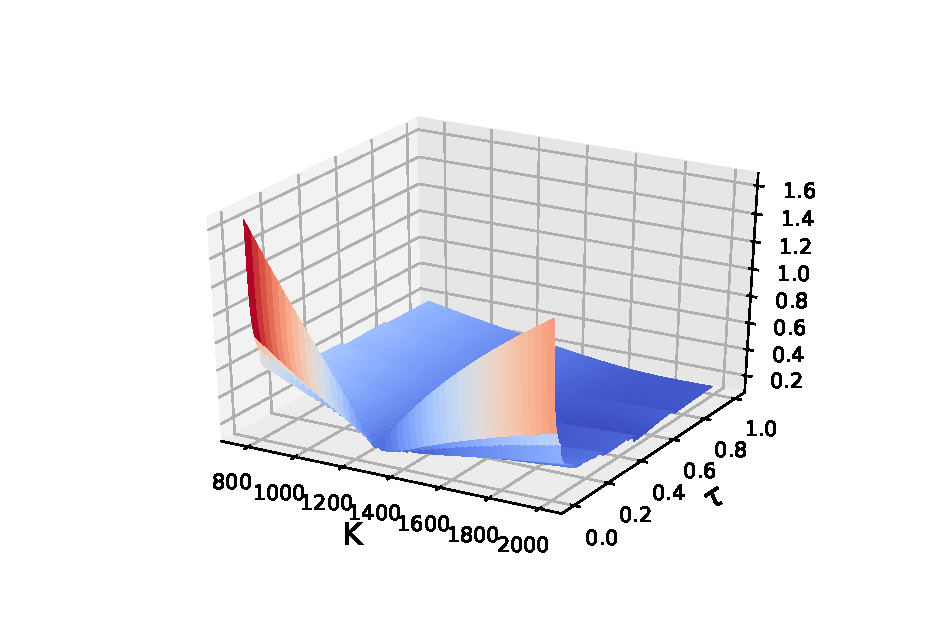
\includegraphics[width=0.8\textwidth]{./figures/ImpVol}
	}
	\subfigure[Price Surface]{
		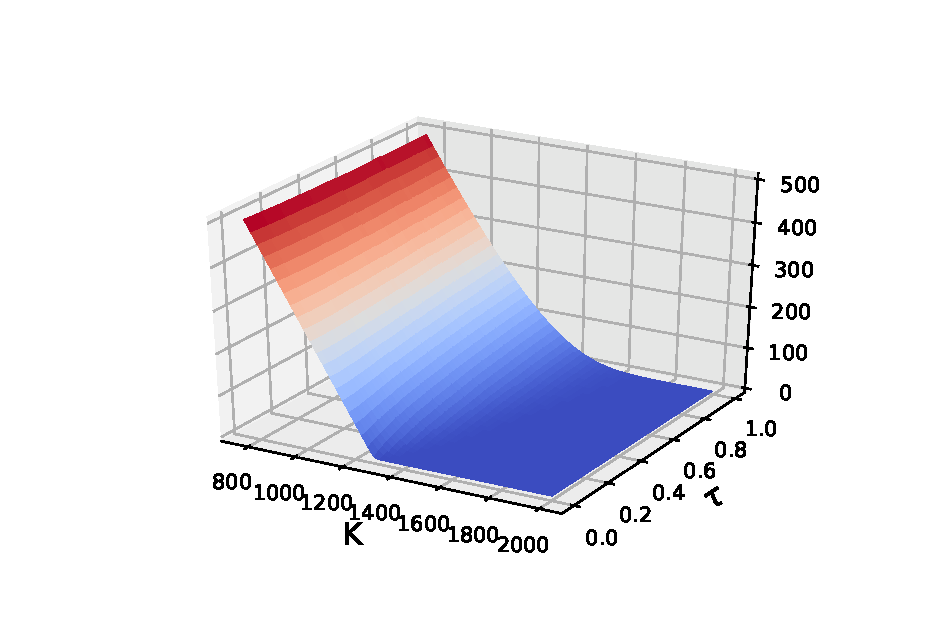
\includegraphics[width=0.8\textwidth]{./figures/Price}
	}
	\caption{The price surface and implied volatility surface calibrated to SP500 index call options on 2012-01-04. The smile is more pronounced for the shorter maturities than the longer maturities, which is consistent with observations from various studies \cite{chance2017bias,rogers2010can} using market data. Interested readers can also refer to \cite{rogers2010can} for some mathematicaly explaination on why the smile becomes more and more flattened as $\tau$ increases.}
	\label{fig:CaliExp}
\end{figure}


\subsubsection{Construction of Training, Testing and Validation Data Sets}
For the experiments in this chapter, we are hedging for a relatively long period (100 business days) until the expiry.  Empirically, we have observed that if we do not update the data-driven model during the hedging period, the performance from the data-driven hedging would be much worse than the performance of the traditional parametric hedging models such as hedging with delta produced by Black-Scholes implied volatility. This is not surprising since market can drastically change during the hedging period which is relatively long and we cannot assume one set of parameter for a data-driven model to be effective for such long period. Lastly, by comparing the performance of local risk model  $\DKLs$, which is updated on a monthly basis,  with those of $\modelN$ and $\model$ ,which are updated on a daily basis in Chapter \ref{sec:LocalComparison}, we can already see the effectiveness of more frequent update.  Therefore, the training and validation data set are updated as we move from one rebalancing date to another rebalancing date. We denote the total risk hedging model as $\modelT$. The detailed description of the model $\modelT$ will be discussed in the following section \ref{sec:TotalModelDes}.

A summary of the construction procedure is given as the following. The detailed procedure of the construction of  training, testing and validation dataset and the overall model building procedure is given in Algorithm \ref{alg:ModelBuilding}.

\begin{steps}
	\item We test on the real market expiries.  The set of all testing expiries is defined as:
	\[
	\mathbf{T}_{AllTest}=\{T^{mkt}|\text{2000-01-01}\leq T^{mkt} \leq \text{2015-08-31}, T^{mkt} \text{  is a market expiry date }\}
	\]
	Namely, we test on all the market observed  expiry date $T$, which are between 2000-01-01 to 2015-08-31. Note that, we have included two crisis periods: the burst of dot-com bubble  period (2000 to 2002) and subprime mortgage crisis period (2007 to 2008). We assume we are on the sell-side of the option trading. 
	
	\item For a testing expiry date $T^{test} \in \mathbf{T}_{AllTest}$, we construct the testing set below:
	\[
	TestSet=\{Scenario(T^{test},K)|\forall K \in \mathbf{K}^{mkt}_{grid}(t_0,T^{test})\}
	\] where $\mathbf{K}^{mkt}_{grid}(t_0,T^{test})$ is the grid of market strikes for expiry $T^{test}$ that can be observed directly from market on the initial date $t_0$. And $t_0$ is 100 business away from $T^{test}$. In other word, the total hedging horizon is $N_H=100$ business days. We build a sequence of models to hedge those testing scenarios with the same expiry date $T^{test}$ and different strikes $K \in \mathbf{K}^{mkt}_{grid}(t_0,T^{test})$. The testing scenario: $Scenario(T^{test},K)$ is constructed using procedure described in Algorithm \ref{alg:TestConstruction}.
	\item On the initial date $t_0$, we prepare the training set  as: 
	\[TrainSet=\{Scenario(T,K)|\forall K \in \mathbf{K}_{grid}(T-\frac{100}{250},T),\forall T \in \mathbf{B}(T_{min},t_0)\}\]
	\[
	\mathbf{B}(T_{min},t_0)=\{ t|t \text{ is a business day},  T_{min}< t <t_0\} 
	\]
 	where $T_{min}$ is the earliest expiry to be included in the training set and  $\mathbf{B}(T_{min},t_0)$ is the set of all business days $t$ with  $T_{min}< t <t_0$. We set $T_{min}$ to be 3 years prior to the intial date of the testing scenarios $t_0$. 
	The grid of strikes $ \mathbf{K}_{grid}(t,T)$ is defined as: $\mathbf{K}_{grid}(t,{T})=\{0=K_0<K_1<\dots<2*K^{mkt}_{max}(t,{T})\}$ with $K_i-K_{i-1}=5, i \geq 1$ and $K^{mkt}_{max}(t,T)$ is defined as the maximum of  strikes we observed in market between between $t$ and  $T$.  
	In other words, we include all training hedging scenarios for which the expiry dates are before $t_0$ and later than $T_{min}$.
	
	The validation set is:
	\[ValSet=\{Scenario(T,K)|T=t_0,  \forall K \in \mathbf{K}_{grid}(T-\frac{100}{250},T)\}\]
	In other words, we include all training hedging scenarios for which the expiry date is $t_0$ as the validation set.
    Note that for training and validation set, we do not require $T$ and $K$ to be observed directly from market.  We train the model based on the training sets. We get the hedging position for the testing scenarios from the data-driven model for $t_0$ only: $\delta^{M}_{t_0,T,K}$.
	

  
	
	\item Similarly, on any rebalancing date $t_j>t_0$,  the training set  and validation set are: 
		\[TrainSet=\{Scenario(T,K)|\forall K \in \mathbf{K}_{grid}(T-\frac{100}{250},T),\forall T \in \mathbf{B}(T_{min},t_j)\}\]
		\[
		\mathbf{B}(T_{min},t_j)=\{ t|t \text{ is a business day},  T_{min}< t <t_j\} 
		\]
	where $\mathbf{B}(T_{min},t_j)$ is the set of all business days $t$ with  $T_{min}< t <t_j$.
	\[ValSet=\{Scenario(T,K)|T=t_j, \forall K  \in \mathbf{K}_{grid}(T-\frac{100}{250},T)\}\]
	We update the model based on the new training set. We get the hedging position from the data-driven model $\modelT$ for $t_j$ only: $\delta^{M}_{t_j,T,K}$. Notice that  the range for the allowed expiries in the training set is extended because $\mathbf{B}(T_{min},t_0) \subset \mathbf{B}(T_{min},t_j)$ when  $t_j>t_0$. Therefore, We have included new data into the training data set. We also validate our model based on most recent scenarios expiring on $t_j$.
\end{steps}


\begin{algorithm}[htp!]
	\DontPrintSemicolon
	
	\SetKwFunction{FMain}{BuildModelForScenarios}
	\SetKwProg{Fn}{Function}{:}{}
	\Fn{\FMain{ $T^{test}$, optType}}{
			\KwIn{ 
				$T^{test}$: A \underline{\textbf{market}} expiry date for the testing hedging scenarios.\newline
				optType: Call or put option. \newline
				\texttt{TestingScenarioGeneration}: The function for generating testing scenarios as in Algorithm \ref{alg:TestConstruction}.\newline
				\texttt{TrainingScenarioGeneration}: The function for generating training scenarios as in Algorithm \ref{alg:Construction}.\newline
			}
			Set  $t_0 \leftarrow T^{test}-\frac{100}{250}$\;
			Extract $\mathbf{t}_{RB}=\{t_0,\dots,t_j,\dots, t_{N_{rb}-1}\}$: the set of \underline{\textbf{rebalancing}} dates sorted in ascending order. Each rebalancing time is $t_j=t_0+j\times \Delta t$ and $\Delta t$ is the gap between the adjacent rebalancing dates.\;
			Extract all market available strikes at $t_0$ for the expiry $T^{test}$ as the grid of strikes:$\mathbf{K}^{mkt}_{grid}(t _0,T^{test})$\;
			TestSet $\leftarrow \texttt{TestingScenarioGeneration}(T^{test}, \text{optType})$\;
			Set $T_{min} \leftarrow t_0-3$: $T_{min}$ is 3 years prior to $t_0$.\;
			\For{$j=0,j<N_{rb},j=j+1$}{
				TrainSet $\leftarrow \emptyset$\;
				Extract $\mathbf{B}(T_{min},t_j)$: the set of all business days between $T_{min}$ and $t_j$.\;
				\For{$T \in \mathbf{B}(T_{min},t_j)$}{
					TrainSubSet$\leftarrow \texttt{TrainingScenarioGeneration}(T, \text{optType})$\;
				$\text{TrainSet} \leftarrow \text{TrainSet}  \cup \text{TrainSubSet}$\;
					
			}
			ValSet$\leftarrow \texttt{TrainingScenarioGeneration}(t_j, \text{optType})$\;
			Bulid model  based on TrainSet\;
			Validate model based on ValSet\;
			Compute the hedging position at $t_j$ for TestSet: $\{\delta^M_{t_j,T,K}|\forall K \in \mathbf{K}^{mkt}_{grid}(t_0,T), T=T^{test}\}$\;
			}
			\KwRet $\{\delta^M_{t,T,K}|\forall t \in \mathbf{t}_{RB},\forall  K \in  \mathbf{K}^{mkt}_{grid}(t_0,{T}),T=T^{test} \}$			
		}
	
	\caption{Function For Building Model To Hedge Scenarios With the Expiry Date $T^{test}$} 
	\label{alg:ModelBuilding}
	\end{algorithm}

\fi


